\documentclass[
11pt, % The default document font size, options: 10pt, 11pt, 12pt
%oneside, % Two side (alternating margins) for binding by default, uncomment to switch to one side
english, % ngerman for German
singlespacing, % Single line spacing, alternatives: onehalfspacing or doublespacing
%draft, % Uncomment to enable draft mode (no pictures, no links, overfull hboxes indicated)
%nolistspacing, % If the document is onehalfspacing or doublespacing, uncomment this to set spacing in lists to single
%liststotoc, % Uncomment to add the list of figures/tables/etc to the table of contents
%toctotoc, % Uncomment to add the main table of contents to the table of contents
%parskip, % Uncomment to add space between paragraphs
%nohyperref, % Uncomment to not load the hyperref package
headsepline, % Uncomment to get a line under the header
%chapterinoneline, % Uncomment to place the chapter title next to the number on one line
%consistentlayout, % Uncomment to change the layout of the declaration, abstract and acknowledgements pages to match the default layout
]{MastersDoctoralThesis} % The class file specifying the document structure

\usepackage[utf8]{inputenc} % Required for inputting international characters
\usepackage[T1]{fontenc} % Output font encoding for international characters

\usepackage{datetime}

\newcommand\hmmax{0}
\newcommand\bmmax{0}

\newdateformat{monthyeardate}{%
\monthname[\THEMONTH], \THEYEAR}

\usepackage{mathpazo} % Use the Palatino font by default

\usepackage[backend=bibtex,style=ieee,natbib=true]{biblatex}

\usepackage{amsmath,amssymb,amsfonts,bm}
\usepackage{scalerel}
\usepackage{mathtools}
\usepackage{graphicx}
\usepackage{float}
\usepackage{mathrsfs}
\usepackage{hyperref}
\usepackage{subcaption}
\usepackage{graphicx}
\usepackage{textcomp}
\usepackage{booktabs}
\usepackage{pifont}
\usepackage{enumitem}
\usepackage{xcolor}

% Bright noticeable placeholders for missing/TODO 
\newcommand{\citeplaceholder}[1]{\textbf{[Cite #1]}}
\newcommand{\placeholderfigure}[1][width=0.8\textwidth]{\fbox{\parbox{#1}{\centering Placeholder for Figure}}}
\newcommand{\placeholdertext}[1]{\textcolor{red}{\textbf{[PLACEHOLDER: #1]}}}

\addbibresource{refs.bib} % The filename of the bibliography

\usepackage[autostyle=true]{csquotes} % Required to generate language-dependent quotes in the bibliography

%----------------------------------------------------------------------------------------
%	MARGIN SETTINGS
%----------------------------------------------------------------------------------------

\geometry{
	paper=a4paper, % Change to letterpaper for US letter
	inner=2.5cm, % Inner margin
	outer=3.8cm, % Outer margin
	bindingoffset=.5cm, % Binding offset
	top=1.5cm, % Top margin
	bottom=1.5cm, % Bottom margin
	%showframe, % Uncomment to show how the type block is set on the page
}

%----------------------------------------------------------------------------------------
%	THESIS INFORMATION
%----------------------------------------------------------------------------------------

\thesistitle{From Sparse Records to Spatial Insights: Clustering and GIS Techniques in Analysis of Named Erratics} % Your thesis title, this is used in the title and abstract, print it elsewhere with \ttitle

\supervisor{Prof. Mahdi \textsc{Agheli}\\Prof. Guanrui \textsc{Li}} % Your supervisor's name, this is used in the title page, print it elsewhere with \supname

\examiner{} % Your examiner's name, this is not currently used anywhere in the template, print it elsewhere with \examname

\degree{Bachelor of Science} % Your degree name, this is used in the title page and abstract, print it elsewhere with \degreename

\author{Ethan \textsc{Chandler}} % Your name, this is used in the title page and abstract, print it elsewhere with \authorname

\addresses{} % Your address, this is not currently used anywhere in the template, print it elsewhere with \addressname

\subject{} % Your subject area, this is not currently used anywhere in the template, print it elsewhere with \subjectname

\keywords{} % Keywords for your thesis, this is not currently used anywhere in the template, print it elsewhere with \keywordnames

\university{\href{https://www.wpi.edu/}{Worcester Polytechnic Institute}} % Your university's name and URL, this is used in the title page and abstract, print it elsewhere with \univname

\department{} % Your department's name and URL, this is used in the title page and abstract, print it elsewhere with \deptname

\group{\href{https://www.wpi.edu/}{Worcester Polytechnic Institute}} % Your research group's name and URL, this is used in the title page, print it elsewhere with \groupname

\faculty{} % Your faculty's name and URL, this is used in the title page and abstract, print it elsewhere with \facname

\AtBeginDocument{
\hypersetup{pdftitle=\ttitle} % Set the PDF's title to your title
\hypersetup{pdfauthor=\authorname} % Set the PDF's author to your name
\hypersetup{pdfkeywords=\keywordnames} % Set the PDF's keywords to your keywords
}

\begin{document}

\frontmatter % Use roman page numbering style (i, ii, iii, iv...) for the pre-content pages

\pagestyle{plain} % Default to the plain heading style until the thesis style is called for the body content

%----------------------------------------------------------------------------------------
%	TITLE PAGE
%----------------------------------------------------------------------------------------

\begin{titlepage}
\begin{center}

% \vspace*{.06\textheight}
\vspace*{1px}
{\scshape\LARGE \univname\par}\vspace{1.5cm} % University name
\textsc{\Large Interactive Qualifying Project}\\[0.5cm] % Thesis type

\HRule \\[0.4cm] % Horizontal line
{\huge \bfseries \ttitle\par}\vspace{0.4cm} % Thesis title
\HRule \\[1.5cm] % Horizontal line
 
\begin{minipage}[t]{0.4\textwidth}
\begin{flushleft} \large
\emph{Author:}\\
\href{https://www.linkedin.com/in/echandler5956f/}{\authorname}\\ % Author name - remove the \href bracket to remove the link
\vspace{0.4cm}
\emph{Supervisor:} \\
\href{https://www.wpi.edu/people/faculty/jcocola}{Professor Jim \textsc{Cocola}}\\
{\small \bfseries Worcester Polytechnic Institute}
\end{flushleft}
\end{minipage}
\begin{minipage}[t]{0.4\textwidth}
\begin{flushright} \large
% \emph{Supervisor:} \\
% \href{https://www.wpi.edu/people/faculty/jcocola}{Professor Jim \textsc{Cocola}}\\
% {\small \bfseries Worcester Polytechnic Institute}\vspace{0.4cm}

\emph{Sponsors:} \\
\href{https://uwaterloo.ca/architecture/profile/j2hutton}{Professor Jane Mah \textsc{Hutton}}\\
{\small \bfseries University of Waterloo}\vspace{0.4cm}

\href{https://www.americanantiquarian.org/}{American Antiquarian Society}\\
{\small \bfseries Worcester, Massachussetts}

\end{flushright}
\end{minipage}\\[1.5cm]


\includegraphics[width=0.2\textwidth]{Images/university.png}

\vfill

\large \textit{An Interactive Qualifying Project submitted in fulfillment of the requirements\\ for the degree of \degreename} at\\[0.3cm] % University requirement text
\groupname \\[2cm] % Research group name and department name
 
\vfill

{\large \monthyeardate\today}\\[4cm] % Date
 
\vfill
\end{center}
\end{titlepage}

%----------------------------------------------------------------------------------------
%	DECLARATION PAGE
%----------------------------------------------------------------------------------------

\begin{declaration}
\addchaptertocentry{\authorshipname} % Add the declaration to the table of contents
\noindent I, \authorname, declare that this Interactive Qualifying Project titled, \enquote{\ttitle} and the work presented in it are my own. I confirm that:

\begin{itemize} 
\item This work was done wholly or mainly while in candidature for a research degree at this University.
\item Where any part of this Interactive Qualifying Project has previously been submitted for a degree or any other qualification at this University or any other institution, this has been clearly stated.
\item Where I have consulted the published work of others, this is always clearly attributed.
\item Where I have quoted from the work of others, the source is always given. With the exception of such quotations, this Interactive Qualifying Project is entirely my own work.
\item I have acknowledged all main sources of help.
\item Where the Interactive Qualifying Project is based on work done by myself jointly with others, I have made clear exactly what was done by others and what I have contributed myself.\\
\end{itemize}
 
\noindent Signed:\\
\rule[0.5em]{25em}{0.5pt} % This prints a line for the signature
 
\noindent Date:\\
\rule[0.5em]{25em}{0.5pt} % This prints a line to write the date
\end{declaration}

\cleardoublepage

%----------------------------------------------------------------------------------------
%	ABSTRACT PAGE
%----------------------------------------------------------------------------------------

\begin{abstract}
\addchaptertocentry{\abstractname} % Add the abstract to the table of contents
Glacial erratics, boulders transported by ice sheets, serve as significant geological markers and potent cultural landmarks across North America. However, systematically analyzing their distribution and significance is challenged by the sparse, heterogeneous, and often qualitative nature of historical and geological records. This paper presents an integrated computational methodology designed to derive spatial and thematic insights from these complex datasets. We combine Geographic Information Systems (GIS) techniques for managing spatial data and calculating proximity metrics (e.g., Haversine distance) with advanced spatial analysis, including density-based clustering (DBSCAN), to identify patterns in erratic distributions. Crucially, we integrate Natural Language Processing (NLP), employing Sentence Transformer embeddings and topic modeling strategies (conceptually based on BERTopic and Latent Dirichlet Allocation - LDA), to extract semantic meaning and thematic structures from associated textual descriptions. We detail the theoretical underpinnings of this pipeline and illustrate its capacity to address specific domain challenges—such as positional ambiguity from historical movement, classification complexity, extreme scale variations, and data sparsity—through in-depth case studies of nine notable North American erratics. This work offers a robust framework for synthesizing diverse data sources, enabling deeper spatial-textual understanding of landscape features characterized by fragmented and challenging records.
\end{abstract}

%----------------------------------------------------------------------------------------
%	ACKNOWLEDGEMENTS
%----------------------------------------------------------------------------------------

\begin{acknowledgements}
\addchaptertocentry{\acknowledgementname} % Add the acknowledgements to the table of contents
The acknowledgments and the people to thank go here, don't forget to include your project advisor\ldots
\end{acknowledgements}

%----------------------------------------------------------------------------------------
%	EXECUTIVE SUMMARY
%----------------------------------------------------------------------------------------

\begin{execSummary}
\addchaptertocentry{\execname}
Glacial erratics – large boulders transported by ancient ice sheets – are significant features across North America, holding clues about past environments and often carrying deep cultural and historical importance. However, understanding their broader patterns and significance is hindered by the nature of the data available: records are often sparse, inconsistent, spread across different sources, and mix geographic locations with historical anecdotes and cultural narratives. Effectively analyzing such fragmented information requires new approaches.

This paper introduces and details a novel computational methodology designed specifically to tackle these challenges. We have developed an integrated system that combines geospatial techniques (mapping, distance calculations) with advanced computational text analysis (Natural Language Processing, or NLP). This allows us to simultaneously analyze the geographic distribution of erratics, identifying spatial clusters and relationships using methods like DBSCAN clustering, while also automatically uncovering key themes and meanings (such as cultural significance, geological descriptions, or historical uses) hidden within the associated textual records using topic modeling and semantic analysis.

The paper explains the theoretical basis of this combined spatial-textual approach and demonstrates its effectiveness through case studies of nine particularly challenging erratics across North America. These examples show how the methodology can handle common problems like rocks that were moved historically, features of vastly different scales, and objects with complex classifications (like a meteorite transported by glaciers).

Ultimately, this research provides a powerful new toolkit for researchers. By systematically integrating sparse spatial and textual data, our methodology enables deeper insights into the geological context, historical relevance, and cultural significance of glacial erratics and similar landscape features characterized by complex and incomplete records. The approach has broader applicability for studies in historical geography, digital humanities, and cultural heritage that grapple with integrating diverse, fragmented data sources.
\end{execSummary}

%----------------------------------------------------------------------------------------
%	LIST OF CONTENTS/FIGURES/TABLES PAGES
%----------------------------------------------------------------------------------------

\tableofcontents % Prints the main table of contents

\listoffigures % Prints the list of figures

\listoftables % Prints the list of tables

%----------------------------------------------------------------------------------------
%	THESIS CONTENT - CHAPTERS
%----------------------------------------------------------------------------------------

\mainmatter % Begin numeric (1,2,3...) page numbering

\pagestyle{thesis} % Return the page headers back to the "thesis" style

% Include the chapters of the thesis as separate files from the Chapters folder
% Uncomment the lines as you write the chapters

\chapter{Introduction}
\label{chapter:intro}
Across the vast landscapes of North America shaped by Pleistocene glaciation, glacial erratics stand as prominent and often enigmatic features. These boulders, ranging from modest stones to colossal megaliths, were transported, sometimes hundreds of kilometers, by continental ice sheets and deposited far from their geological origins as the ice retreated \cite{Flint1971, Benn2010}. Their significance is twofold. Scientifically, they serve as direct physical evidence of past ice extent, flow directions, and erosional processes, providing invaluable data points for reconstructing Quaternary environments \cite{Cuffey2010}. Culturally, many named erratics have become deeply embedded in human history and perception, functioning as sacred sites in Indigenous traditions, navigational landmarks for travelers, boundary markers in colonial settlements, sources of local folklore, and even national symbols \cite{Seelye1997, Lenik2009, Dempsey1997}.

Despite their ubiquity and importance, conducting large-scale, systematic analyses of named glacial erratics presents significant methodological hurdles, primarily stemming from the nature of the available data. Unlike standardized geological surveys, information about named erratics is often scattered across diverse sources: historical texts, geological reports, archaeological surveys, local historical society records, oral histories, and digital databases of varying quality. Consequently, the data corpus is characterized by sparsity and heterogeneity \cite{Gregory2013}. Records may be geographically biased, with dense documentation in some regions (like New England) and sparse information in others. Data quality varies dramatically; some erratics have precise geological descriptions and coordinate locations, while others are documented through vague textual accounts or approximate locations. Furthermore, the data often mixes quantitative metrics (size, elevation) with qualitative, unstructured text (historical narratives, cultural significance), and must account for temporal changes, as many significant erratics have been moved, fractured, or re-contextualized over time (Section \ref{chapter:cases}).

Addressing this data challenge requires computational methods capable of integrating and analyzing these disparate, multi-modal data sources effectively. There is a need for a robust framework that can handle spatial uncertainty, synthesize quantitative spatial relationships with qualitative textual information, and identify meaningful patterns despite data sparsity and noise. This paper aims to address this gap by pursuing three primary objectives: (1) To develop and rigorously detail an integrated computational methodology combining geospatial analysis and Natural Language Processing (NLP) specifically tailored for the study of North American named glacial erratics. (2) To demonstrate, through theoretical exposition and practical considerations, how this methodology directly confronts key challenges inherent in the domain, including data sparsity, locational ambiguity, classification complexity involving both geological and cultural facets, and the representation of non-standard features like boulder fields or scale outliers. (3) To illustrate the rationale and necessity of the methodology's specific components through in-depth case studies of nine particularly complex and informative erratic examples that drove its design.

The methodology presented herein (detailed in Section \ref{chapter:method}) leverages a Geographic Information System (GIS) framework built upon a spatially-enabled database (conceptually PostgreSQL/PostGIS). This foundation supports the integration of erratic data with relevant contextual geographic layers (hydrology, settlements, transport networks, Indigenous territories). Spatial analysis techniques are employed to compute geodesic proximity metrics (using the Haversine formula \cite{Sinnott1984}) and to identify spatial patterns through density-based clustering (DBSCAN \cite{Ester1996}). Crucially, these geospatial methods are coupled with advanced NLP techniques applied to the textual corpus associated with each erratic. We utilize pre-trained Sentence Transformer models \cite{Reimers2019} to generate semantic vector embeddings, capturing nuanced meaning beyond keywords. These embeddings facilitate unsupervised topic discovery using approaches conceptually grounded in BERTopic \cite{Grootendorst2022} (embedding clustering) and Latent Dirichlet Allocation (LDA \cite{Blei2003}) (probabilistic topic modeling), allowing for the identification and classification of latent thematic content within the descriptions.

The development of this integrated pipeline was not purely theoretical but was substantially informed by confronting the complexities of real-world examples. Section \ref{chapter:cases} presents detailed case studies of nine prominent North American erratics (including Plymouth Rock, Okotoks "Big Rock", the Willamette Meteorite, Babson's Boulders, and others). These cases are presented not merely as applications, but as critical methodological drivers. Their unique characteristics—histories of movement and fragmentation, extreme scale, contested classifications, collective versus individual nature, and deep, specific cultural meanings—exposed the limitations of simpler analytical approaches and necessitated the development of the more sophisticated and flexible methods detailed in Section \ref{chapter:method}.

This paper proceeds as follows: Section \ref{chapter:cases} provides the in-depth case studies that highlight the methodological challenges. Section \ref{chapter:method} details the theoretical foundations and algorithmic components of the integrated geospatial and NLP analysis pipeline designed to address these challenges. Section \ref{chapter:results} presents the outcomes of applying this methodology to the broader dataset, discussing the emergent spatial and thematic patterns. Finally, Section \ref{chapter:conclusion} summarizes the contributions and suggest avenues for future research in the computational analysis of complex landscape features like glacial erratics.


\chapter{Case Studies}
\label{chapter:cases}

\section{Defining the Need for Methodological Nuance}
\label{sec:nuance}

The study of named glacial erratics across North America presents a fascinating intersection of geology, history, culture, and geography. These lithic travelers, carried vast distances by Pleistocene ice sheets and deposited often incongruously upon the landscape, serve not only as tangible evidence of past glacial dynamics but also as focal points for human interaction, belief systems, and historical narratives \cite{Flint1971, Benn2010}. While a systematic, large-scale analysis promises novel insights into patterns of distribution, cultural significance, and geological context, such an endeavor quickly confronts the inherent complexity and heterogeneity of the data associated with these unique features.

Our research employs a sophisticated AI/ML spatial analysis pipeline, integrating diverse geospatial datasets, proximity calculations, and advanced Natural Language Processing (NLP) techniques to classify and contextualize named erratics (as detailed in Section III: Methodology). However, the development and refinement of this pipeline were significantly shaped by encounters with specific erratics that defied straightforward categorization or analysis. These "outliers" or exceptional cases presented unique methodological challenges stemming from factors such as positional ambiguity due to historical movement, complex or contested classifications, extreme physical scale, the representation of collections versus single objects, and profound cultural significance often unevenly documented or requiring specialized interpretation.

This section delves into detailed case studies of nine prominent North American glacial erratics. These specific examples—Plymouth Rock, Dighton Rock, Okotoks "Big Rock" Erratic, Willamette Meteorite, Babson's Boulders, Madison Boulder, Bleasdell Boulder, Rollstone Boulder, and Judges Cave—were selected not only for their individual renown but because they collectively encapsulate the spectrum of challenges that necessitated significant adaptations to our data modeling, analytical algorithms, and classification schemes. By examining the historical, cultural, and physical particularities of each case, we illustrate \emph{why} a simplistic or standardized analytical approach is insufficient. These case studies serve as critical precursors to the subsequent Methodology section, demonstrating the empirical grounding for the specific technical solutions implemented in our pipeline to handle ambiguity, complexity, scale, and the rich tapestry of human interaction woven around these geological landmarks. Understanding these exceptions is fundamental to appreciating the robust, flexible, and context-aware analytical framework ultimately required for this research domain \cite{Cuffey2010, Delcourt1991}.

\section{Individual Cases}
\label{sec:individual_cases}

\subsection{Plymouth Rock (Plymouth, Massachusetts): A Symbol Moved, Fractured, and Reified}
\label{subsec:plymouth}

Perhaps no glacial erratic in North America carries the symbolic weight of Plymouth Rock, enshrined in national mythology as the disembarkation point of the Mayflower Pilgrims in 1620 \cite{Seelye1997}. Yet, from a geo-analytical perspective, it represents a profound case of positional ambiguity, physical alteration, and the dominance of cultural narrative over geological fact, posing significant challenges for standardized data capture and analysis.

\textbf{Historical Context and Movement:} The historical record linking the Pilgrims directly to this specific rock is tenuous, emerging decades after the landing, primarily through the testimony of Elder Thomas Faunce in 1741 \cite{Seelye1997}. The rock, originally situated at the waterline of Plymouth Harbor, became an object of veneration and, consequently, modification. In 1774, during revolutionary fervor, an attempt to move the boulder resulted in its accidental splitting. The upper portion was relocated to the Town Square, later moved again near Pilgrim Hall, and finally rejoined with the base portion (which itself had been moved slightly for wharf construction) under the present-day granite portico in 1920 \cite{Seelye1997}. This complex history means Plymouth Rock has occupied at least four distinct locations, and the currently displayed artifact is only a fragment of the original Dedham granodiorite boulder \cite{Emerson1917}.

\textbf{Physical Characteristics and Alteration:} Estimates suggest the original boulder may have weighed upwards of 20 tons, whereas the current fragment is considerably smaller \cite{Emerson1917}. Decades of souvenir hunting further reduced its size before protective measures were enacted. Its geological origin is traced to exposures likely miles away, consistent with glacial transport by the Laurentide Ice Sheet \cite{Emerson1917}. However, its primary identity is now cultural, not geological.

\textbf{Methodological Challenges:}
\begin{itemize}
    \item \textbf{Positional Ambiguity:} Which location represents Plymouth Rock in our database? The original, estimated waterline position? The 1774 Town Square location? The Pilgrim Hall location? The current portico location? Each choice drastically alters proximity calculations to historical shorelines, settlements, and other features. Our pipeline needed a mechanism to store \emph{multiple} coordinate pairs associated with a single entity, flagged by time period or type (e.g., \texttt{location\_original\_estimated}, \texttt{location\_1774}, \texttt{location\_current}).
    \item \textbf{Size and Integrity:} Recording the \texttt{size\_meters} is problematic. Do we record the estimated original size, or the size of the current fragment? The discrepancy impacts its placement within our \texttt{size\_category} classification (e.g., "Medium" vs. "Large"). We needed to implement fields for both \texttt{size\_current\_estimated} and \texttt{size\_original\_estimated}, along with confidence flags.
    \item \textbf{Classification Dominance:} While geologically an erratic, its overwhelming significance is cultural and symbolic ("National Monument," "Symbolic Landmark"). Our NLP classification, analyzing text descriptions, overwhelmingly flags it for cultural significance, potentially masking its more modest geological attributes. The \texttt{usage\_type} array needed to accommodate multiple tags like \texttt{['Symbolic', 'Monument', 'Geological']}, and the \texttt{cultural\_significance\_score} derived from NLP required careful calibration to handle such extreme cases.
    \item \textbf{Data Integrity:} Much of the rock's narrative is based on tradition rather than verifiable contemporary accounts. This highlights the need for associating source reliability or confidence levels with historical data entries within the database.
\end{itemize}

\textbf{Pipeline Implications:} Plymouth Rock forced the development of data structures capable of handling temporal-spatial ambiguity (multiple locations over time), fragmented objects (multiple size estimates), and the nuanced interplay between geological classification and intense cultural overlay. It necessitated flexible location referencing in proximity analyses (allowing users to choose historical vs. current context) and sophisticated NLP handling to balance symbolic weight with other attributes.

\subsection{Dighton Rock (Berkley, Massachusetts): A Canvas of Contested Histories, Relocated}
\label{subsec:dighton}

Dighton Rock, a sandstone boulder famed for its dense and enigmatic petroglyphs, presents challenges related to contested interpretations, historical relocation, and the difficulty of classifying its primary significance. Originally located in the tidal Taunton River, its inscriptions have fueled centuries of speculation about pre-Columbian trans-oceanic contact \cite{Lenik2009, Delabarre1928}.

\textbf{Historical Context and Petroglyphs:} The \textasciitilde40-ton boulder, likely deposited by glacial action in the riverbed, bears carvings whose origins remain debated. Attributions range from Indigenous peoples (Wampanoag or earlier groups), to Portuguese explorers (Miguel Corte-Real), Norsemen, Chinese sailors, and even Phoenicians \cite{Lenik2009, Pohl1950}. Colonial accounts, like that of Rev. John Danforth in 1680 and Cotton Mather in 1712, document early European awareness and attempts at interpretation \cite{Lenik2009, Delabarre1928}. This long history of contested interpretation makes classifying its "cultural significance" complex.

\textbf{Physical Characteristics and Movement:} The rock is composed of greywacke sandstone, atypical for the immediate region, confirming its erratic nature \cite{Delabarre1928}. Crucially, in 1963, the boulder was removed from its tidal riverbed location to protect it from vandalism and erosion. It was eventually housed in a purpose-built museum within Dighton Rock State Park, located on the nearby riverbank \cite{Lenik2009, MassDCRDighton}.

\textbf{Methodological Challenges:}
\begin{itemize}
    \item \textbf{Positional Ambiguity (Context Shift):} Similar to Plymouth Rock, Dighton Rock exists in two key locations: its original, intertidal context and its current museum setting. Proximity analysis yields vastly different results depending on the chosen coordinates. Calculating \texttt{nearest\_water\_body\_dist} using the museum location yields a small, potentially misleading value compared to its original \emph{in situ} riverine position. The historical context—being repeatedly submerged and exposed by tides—is lost if only the current location is used. Our pipeline required the ability to store and differentiate between \texttt{location\_original} and \texttt{location\_current\_museum}, and allow analysis toggles based on research questions (e.g., analyzing historical accessibility vs. modern).
    \item \textbf{Classification of Significance:} How should Dighton Rock be primarily classified? As a geological erratic? An archaeological site? A historical curiosity? A locus of specific cultural (Indigenous) heritage amidst speculative claims? Our NLP analysis of descriptive texts needed to capture this multifaceted identity. The \texttt{usage\_type} array might include \texttt{['Petroglyph Site', 'Archaeological', 'Historical Landmark', 'Indigenous Significance', 'Geological']}. Deriving a single \texttt{cultural\_significance\_score} becomes challenging due to the \emph{contested} nature of its primary meaning.
    \item \textbf{Inscriptions:} The presence of detailed inscriptions (\texttt{has\_inscriptions} = True) is a key attribute, requiring specific handling in the database and potentially influencing NLP topic modeling if inscription details are textually described.
    \item \textbf{Environmental Context:} The original tidal environment was crucial to its historical visibility and interpretation (and potential degradation). Standard \texttt{elevation} and \texttt{geomorphology} fields based on its current museum location fail to capture this vital original context. Supplemental fields or descriptive flags were needed.
\end{itemize}

\textbf{Pipeline Implications:} Dighton Rock underscored the need for dual-location tracking (original vs. current) and the ability to perform proximity analyses based on context-dependent coordinates. It highlighted the challenges of classifying objects with deeply contested historical interpretations and the need for NLP models sensitive to nuances beyond simple topic identification. The environmental context shift also prompted consideration of storing original environmental setting data where available and relevant.

\subsection{Okotoks "Big Rock" Erratic (Okotoks, Alberta): An Outlier of Immense Scale and Sacred Significance}
\label{subsec:okotoks}

The Okotoks Erratic, known locally as "Big Rock," is a spectacular example of a glacial erratic notable for its immense size and its deep significance within Blackfoot (Siksika) traditional narratives \cite{AlbertaOkotoks, Dempsey1997}. Located on the relatively flat prairie west of Okotoks, Alberta, this quartzite behemoth presents a classic "outlier" problem for quantitative analysis and demands culturally sensitive data handling.

\textbf{Geological Context and Scale:} Part of the Foothills Erratics Train, Big Rock was transported hundreds of kilometers from the Jasper area of the Canadian Rockies by the Laurentide Ice Sheet \cite{AlbertaOkotoks, Stalker1973}. Composed of layered quartzite, it measures approximately 41 by 18 meters and stands 9 meters tall, with an estimated mass of 16,500 tonnes \cite{AlbertaOkotoks}. Its sheer size makes it one of the largest known glacial erratics globally. It has also fractured into two main pieces, likely due to frost weathering over millennia \cite{Dempsey1997}.

\textbf{Cultural Significance:} For the Blackfoot people, Big Rock is intrinsically linked to the stories of Napi (Old Man), the trickster figure and creator \cite{Dempsey1997, Klassen1995}. One prominent story explains Napi gave his robe to the rock on a hot day, later asked for it back when the weather turned cold, and was chased by the rolling rock after refusing Napi's request. Napi struck the rock with help from bats, splitting it in two \cite{Dempsey1997}. This narrative embeds the rock within a sacred geography and cosmology, marking it as far more than just a geological feature. It is designated as a Provincial Historic Resource \cite{AlbertaOkotoks}.

\textbf{Methodological Challenges:}
\begin{itemize}
    \item \textbf{Scale Outlier:} Big Rock's mass and dimensions far exceed those of most other named erratics in North America. If included directly in statistical analyses of size (e.g., calculating mean or standard deviation of \texttt{size\_meters} or volume), it would heavily skew the results. Our \texttt{size\_category} classification needed refinement; simply having "Small, Medium, Large" was insufficient. A "Monumental" or "Mega-Erratic" category, potentially defined by specific thresholds or percentile cutoffs, was required to handle such extremes without distorting the overall distribution \cite{Cuffey2010}. Statistical analyses needed options for outlier detection and robust methods (e.g., using median instead of mean).
    \item \textbf{Cultural Significance Encoding:} Capturing the depth of Blackfoot significance required more than a simple keyword tag. Our NLP analysis needed to be trained or fine-tuned to recognize and appropriately weight descriptions related to Indigenous oral traditions, sacredness, and specific mythological figures (like Napi). The \texttt{cultural\_significance\_score} needed to reflect this deep, specific cultural embedding, potentially using rule-based adjustments alongside NLP outputs. The connection to the broader Foothills Erratics Train, also culturally significant, needed representation \cite{Klassen1995}.
    \item \textbf{Fragmentation:} Although often referred to as "Big Rock," it's technically fragmented. Our data model needed clarity on whether to represent it as a single entity with notes on fragmentation or as two closely related entities, impacting spatial queries and proximity calculations at very fine scales.
\end{itemize}

\textbf{Pipeline Implications:} Okotoks Big Rock forced the implementation of robust outlier handling techniques in statistical summaries and classification schemes related to physical size (\texttt{size\_category}, \texttt{size\_meters}). It highlighted the critical need for culturally sensitive NLP capabilities and data fields capable of capturing the nuances of Indigenous sacred significance beyond simple topical classification. The fragmentation issue also reinforced the need for clear guidelines on representing composite or fractured features.

\subsection{Willamette Meteorite (West Linn, Oregon / New York City): An Extraterrestrial Erratic with Contested Ownership and Sacred Status}
\label{subsec:willamette}

The Willamette Meteorite presents a unique classification challenge: it is undeniably extraterrestrial in origin but experienced geological transport processes akin to terrestrial erratics, likely involving both glacial ice and cataclysmic floods \cite{AMNHWillamette, Pasek2008}. Its status as a sacred object to the Clackamas Chinook people adds further layers of complexity regarding ownership, location, and interpretation.

\textbf{Origin and Transport:} This 15.5-ton iron-nickel meteorite, the largest found in North America, originated in the asteroid belt \cite{AMNHWillamette}. Its journey to Oregon's Willamette Valley remains debated but likely involved landing in western Canada or Montana during the last ice age. It was then incorporated into the Cordilleran Ice Sheet, transported southward, and likely rafted by icebergs during the Missoula Floods that scoured the region between 15,000 and 13,000 years ago, finally coming to rest near modern-day West Linn \cite{Pasek2008, Bretz1969}. This complex transport history involving both glacial ice and megafloods blurs the lines of typical glacial erratic deposition.

\textbf{Discovery and Cultural Significance:} The meteorite was known to the Clackamas Chinook people, who called it \emph{Tomanowos} ("Visitor from the Moon" or "Heavenly Visitor") and revered it for its spiritual power, using rainwater collected in its hollows for rituals \cite{statesmanjournalPiecesSacred, ourtimebdTomanowosMeteorite}. It was "rediscovered" by settler Ellis Hughes in 1902, who secretly moved it onto his own land, sparking a legal battle eventually won by the Oregon Iron and Steel Company, on whose land it had originally rested \cite{AMNHWillamette}. It was sold and eventually donated to the American Museum of Natural History (AMNH) in New York City in 1906, where it remains \cite{AMNHWillamette}. The Confederated Tribes of Grand Ronde, successors to the Clackamas, have long sought its repatriation, resulting in a landmark 2000 agreement allowing continued museum display but guaranteeing tribal access for religious and cultural purposes \cite{statesmanjournalPiecesSacred, ourtimebdTomanowosMeteorite}.

\textbf{Methodological Challenges:}
\begin{itemize}
    \item \textbf{Classification Ambiguity:} Is \emph{Tomanowos} a "glacial erratic"? It was transported by ice and water associated with glaciation, but its origin is extraterrestrial. Our pipeline's standard classification based on \texttt{rock\_type} (expecting terrestrial igneous, metamorphic, or sedimentary rocks) failed. We needed a special classification flag or category (e.g., \texttt{geological\_type} = 'Meteorite (Glacially Transported)').
    \item \textbf{Inapplicable Metrics:} Calculating \texttt{estimated\_displacement\_dist} based on terrestrial bedrock sources is impossible. This key analytical field, designed for standard erratics, yielded nonsensical results. We needed to flag entities like this to exclude them from such specific geological analyses or develop alternative metrics related to flood path modeling.
    \item \textbf{Dual Location and Ownership Context:} Like Plymouth and Dighton Rocks, it has a significant original location (West Linn, OR) and a current one (AMNH, NYC). Proximity analyses are location-dependent. Furthermore, the contested ownership and eventual agreement are crucial contextual elements. Our data model needed fields to capture original location, current location, and complex custodial/cultural stewardship arrangements.
    \item \textbf{Sacred Significance and NLP:} The deep sacredness to the Clackamas, embodied in the name \emph{Tomanowos} and associated rituals, required careful handling. NLP analysis needed to identify and prioritize this Indigenous cultural significance, potentially linking it to broader regional Indigenous cosmologies related to celestial events or powerful natural features \cite{ourtimebdTomanowosMeteorite}. The \texttt{cultural\_significance\_score} needed to strongly reflect this documented sacred status.
\end{itemize}

\textbf{Pipeline Implications:} The Willamette Meteorite forced a fundamental reconsideration of the definition of "erratic" within the project scope, necessitating new classification categories (\texttt{geological\_type}). It demonstrated the limitations of standardized geological metrics (\texttt{estimated\_displacement\_dist}) for exceptional cases. It reinforced the need for multi-location tracking and added the complexity of representing ongoing cultural stewardship and contested histories. The case underscored the ethical imperative of prioritizing and accurately representing Indigenous cultural significance identified through NLP and other sources \cite{statesmanjournalPiecesSacred}.

\subsection{Babson's Boulders (Gloucester, Massachusetts): A Dispersed Collection Challenging Entity Definition}
\label{subsec:babson}

Located within the historically bleak and fascinating landscape of Dogtown Common on Cape Ann, Babson's Boulders represent not a single erratic but a collection of dozens of glacially deposited boulders deliberately inscribed with inspirational mottoes by philanthropist Roger Babson during the Great Depression \cite{Moore2005, wburMysteriousBoulders}. This presents a significant challenge to database schemas and spatial analysis techniques designed around individual point features.

\textbf{Historical Context:} Dogtown Common, once a thriving inland settlement in the 17th and 18th centuries, had become largely abandoned and overgrown by the 19th century, known for its poverty, isolation, and folklore involving witches and wild dogs \cite{Moore2005, Babson1940}. During the 1930s, Roger Babson, a successful economist and statistician, commissioned unemployed Finnish stonecutters to carve mottoes ("Keep Out Of Debt," "Help Mother," "Prosperity Follows Service") onto numerous large granite and gneiss erratics scattered across the common \cite{wburMysteriousBoulders}. His motives were partly philanthropic (providing work) and partly didactic, intending the inscriptions as enduring lessons for visitors \cite{Moore2005}.

\textbf{Physical Characteristics:} Dogtown is littered with thousands of glacial erratics, remnants of the Laurentide Ice Sheet's passage over the local granite bedrock. Babson selected dozens of these existing boulders, varying in size, for his project \cite{wburMysteriousBoulders}. They are not concentrated in one spot but distributed across a significant area of the common (over 3,000 acres).

\textbf{Methodological Challenges:}
\begin{itemize}
    \item \textbf{Entity Definition (One vs. Many):} How should "Babson's Boulders" be represented in a spatial database? As a single point (e.g., a centroid of the inscribed boulders)? As a polygon encompassing the area where they are found? Or as individual records for each of the \textasciitilde30-40 inscribed boulders?
        \begin{itemize}
            \item \emph{Single Point/Polygon:} Simplifies database entry but loses crucial detail. Proximity analysis to this single point/polygon becomes less meaningful for understanding access to individual boulders. Clustering analysis might incorrectly group this single representation with other distinct erratics.
            \item \emph{Individual Records:} Most accurate representation but significantly increases data entry effort. Requires unique identifiers and coordinates for each inscribed boulder. Allows for fine-grained analysis but complicates queries seeking information about the "collection" as a whole.
        \end{itemize}
    \item \textbf{Clustering Analysis:} If represented as individual points, the Babson Boulders would naturally form a tight spatial cluster in analyses like DBSCAN. This is accurate locally but could be misinterpreted as a single geological event or feature if not contextualized as a deliberately created \emph{collection} of \emph{separate} erratics. The analysis output needs flagging to indicate this is an "artificial" or "curated" cluster.
    \item \textbf{Classification:} While individually geological erratics, their primary modern significance derives from the historical act of inscription and Babson's social project. The \texttt{usage\_type} needs to reflect this duality: \texttt{['Inscription Site', 'Historical Landmark', 'Geological', 'Art Installation']}. NLP analysis would focus on the content and context of the inscriptions and Babson's history.
    \item \textbf{Data Acquisition:} Precisely locating and documenting each inscribed boulder requires significant fieldwork or reliance on potentially incomplete existing datasets (e.g., from local trail maps or historical societies) \cite{wburMysteriousBoulders}.
\end{itemize}

\textbf{Pipeline Implications:} Babson's Boulders highlighted the critical "unit of analysis" problem for collections or clusters of related features. It necessitated developing strategies within the database schema and analytical scripts to handle both collection-level representation (e.g., using polygons or parent-child relationships) and individual feature representation. It required specific parameters or post-processing steps in clustering algorithms to avoid misinterpreting curated collections as purely natural clusters. The need for clear metadata defining \emph{how} such collections are represented became paramount.

\subsection{Madison Boulder (Madison, New Hampshire): Handling Another Giant}
\label{subsec:madison}

Madison Boulder, located in a dedicated Natural Area in New Hampshire, stands as another testament to the immense power of glacial transport and, like Okotoks Big Rock, presents challenges related to extreme scale \cite{Goldthwait1925, NHMadisonBoulder}. It is renowned as one of the largest known glacial erratics in North America.

\textbf{Geological Context and Scale:} This colossal boulder is composed of Conway granite, a distinctive local bedrock type, confirming its relatively shorter (though still significant) transport distance compared to erratics like Okotoks \cite{Goldthwait1925, NPSMadisonBoulder}. Its dimensions are roughly 25 meters long, 9 meters high, and 11 meters wide, with an estimated weight of approximately 4,662 tonnes (often cited as over 5,000 tons) \cite{NHMadisonBoulder, NPSMadisonBoulder}. It rests partially buried in a forested setting, deposited as the Laurentide Ice Sheet retreated around 14,000 years ago \cite{Goldthwait1925}.

\textbf{Historical and Cultural Context:} While lacking the deep, specific Indigenous narratives associated with Okotoks (though the region is ancestral Abenaki territory), Madison Boulder has been a known landmark and natural curiosity for centuries, attracting visitors and geological interest \cite{NHMadisonBoulder}. It was designated a National Natural Landmark in 1970 \cite{NPSMadisonBoulder}. Its significance is primarily geological and as a local point of interest.

\textbf{Methodological Challenges:}
\begin{itemize}
    \item \textbf{Scale Outlier:} Madison Boulder reinforces the challenge posed by Okotoks: its massive size places it far outside the typical range for named erratics. It necessitates the "Monumental" \texttt{size\_category} and requires outlier-robust statistical methods to avoid distorting analyses of average erratic size, volume, or weight across the dataset \cite{Cuffey2010}.
    \item \textbf{Precise Measurement Difficulty:} Due to its partial burial and irregular shape, obtaining precise volume and weight estimates is challenging, leading to slightly varying figures in different sources \cite{NHMadisonBoulder, NPSMadisonBoulder}. This highlights the need for \texttt{confidence\_score} fields associated with physical measurements, especially for very large or awkwardly situated erratics.
    \item \textbf{Comparison with Okotoks:} While both are scale outliers, Madison Boulder's granite composition and likely shorter transport distance contrast with Okotoks' quartzite and long-distance journey within an erratic train \cite{AlbertaOkotoks, Goldthwait1925}. This comparison underscores the need for the pipeline to capture not just size but also \texttt{rock\_type}, \texttt{estimated\_displacement\_dist}, and geological context (e.g., part of a known train vs. solitary giant) to enable meaningful comparative analysis even among outliers.
\end{itemize}

\textbf{Pipeline Implications:} Madison Boulder provides a crucial second data point confirming the necessity of specialized handling for mega-erratics within the database and analytical routines. It reinforces the need for a \texttt{size\_category} scheme that includes a "Monumental" class and statistical methods robust to extreme values. It also highlights the importance of capturing geological context alongside size to differentiate between different types of large erratics and the value of confidence indicators for measurements.

\subsection{Bleasdell Boulder (Trenton, Ontario): Dealing with Data Sparsity and Regional Variation}
\label{subsec:bleasdell}

The Bleasdell Boulder, located within the Bleasdell Boulder Conservation Area near Trenton, Ontario, is recognized as one of Canada's largest known glacial erratics \cite{LTCBleasdell, Chapman1984}. While a significant local landmark, its documentation illustrates the challenge of data heterogeneity and sparsity often encountered when moving beyond the most famous North American erratics.

\textbf{Geological Context and Size:} Composed of Precambrian granite gneiss, the Bleasdell Boulder measures approximately 13.4 meters long, 7.3 meters wide, and 6.7 meters high \cite{LTCBleasdell}. Its estimated weight is around 2,000 tonnes. It was transported by the Laurentide Ice Sheet from the Canadian Shield, likely hundreds of kilometers to the north, and deposited as the ice retreated \cite{Chapman1984}.

\textbf{Historical and Cultural Context:} The boulder has been a known landmark for local inhabitants, including First Nations (likely Mississauga or preceding groups) and later European settlers, for a considerable time \cite{Chapman1984}. It gained wider recognition and protection when the surrounding land was acquired for conservation in the mid-20th century \cite{LTCBleasdell}. Compared to Plymouth Rock or Dighton Rock, however, detailed historical accounts, specific Indigenous narratives, or extensive folklore directly attached to this \emph{specific} boulder appear less prevalent or less widely documented in easily accessible sources.

\textbf{Methodological Challenges:}
\begin{itemize}
    \item \textbf{Data Sparsity and Heterogeneity:} While basic geological data (size, rock type, location) are available, obtaining rich, detailed historical narratives, documented pre-colonial usage, or extensive cultural significance information proved more challenging than for some US counterparts with longer colonial documentation histories or more widely studied Indigenous contexts \cite{Delcourt1991}. This unevenness in available data is a common problem in large-scale North American studies.
    \item \textbf{Impact on NLP and Classification:} When textual descriptions (\texttt{description}, \texttt{cultural\_significance}, \texttt{historical\_notes}) are sparse or generic ("large local landmark"), NLP topic modeling and classification have less material to work with. This can lead to less specific topic assignments or lower confidence scores for \texttt{cultural\_significance\_score}. The pipeline must be able to handle records with missing or minimal textual data gracefully, perhaps assigning default categories or flagging them for manual review.
    \item \textbf{Regional Variation:} The nature and availability of historical records often vary significantly between regions (e.g., Eastern US vs. Central Canada vs. Pacific Northwest). A pipeline designed primarily around well-documented New England sites might struggle with data patterns from other regions. The system needed robustness to handle varying levels of detail and types of information sources across the continent.
    \item \textbf{Confidence Flagging:} The potential for undocumented significance means analyses based \emph{only} on available data might underestimate the boulder's historical or cultural importance. This reinforces the need for methodological transparency, acknowledging limitations imposed by data availability and potentially using \texttt{confidence\_score} fields not just for measurements but also for qualitative assessments like cultural significance when based on limited evidence.
\end{itemize}

\textbf{Pipeline Implications:} The Bleasdell Boulder case highlighted the pervasive issue of data sparsity and regional heterogeneity in historical and cultural documentation for many erratics. It necessitated building fault tolerance into the NLP pipeline to handle missing or minimal text and ensuring that classification outputs reflect data confidence. It emphasized the need to integrate diverse regional data sources and be transparent about analysis limitations stemming from uneven data coverage.

\subsection{Rollstone Boulder (Fitchburg, Massachusetts): Relocation and Reassembly of a Community Symbol}
\label{subsec:rollstone}

The Rollstone Boulder shares similarities with Plymouth Rock and Dighton Rock in its history of movement, but adds the complexity of fragmentation followed by deliberate reassembly \cite{googleLewistonEvening, telegramWorcesterCounty}. Originally perched atop Rollstone Hill in Fitchburg, this large porphyritic granite boulder became a cherished local symbol, only to be threatened by quarrying operations.

\textbf{Geological Context and Original Location:} The \textasciitilde110-ton boulder is composed of porphyritic granite, geologically distinct from Rollstone Hill itself (composed of gneiss), confirming its status as an erratic transported by the Laurentide Ice Sheet \cite{mindatMineralsRollstone, Hitchcock1841}. Its prominent position on the hilltop made it a natural landmark.

\textbf{Historical Context, Movement, and Reassembly:} As quarrying encroached on Rollstone Hill in the late 19th and early 20th centuries, local citizens grew concerned for the boulder's fate \cite{googleLewistonEvening, telegramWorcesterCounty}. Notably, Fitchburg naturalist James F. D. Garfield advocated for its preservation \cite{googleLewistonEvening}. In 1929-1930, a plan was enacted: the boulder was carefully blasted into manageable pieces, transported down the hill, and meticulously reassembled in a small park (Crocker Field, later relocated slightly to the Upper Common) in downtown Fitchburg, where it stands today as a monument \cite{googleLewistonEvening, telegramWorcesterCounty}.

\textbf{Methodological Challenges:}
\begin{itemize}
    \item \textbf{Positional Ambiguity (Dual Context):} Like Plymouth and Dighton Rocks, the Rollstone Boulder has two critically important locations: its original commanding position on Rollstone Hill and its current location in the downtown park. Analyzing its \texttt{elevation\_category} or proximity to natural features makes sense only relative to the \emph{original} location. Analyzing its \texttt{accessibility\_score} (based on modern roads/settlements) or its role as a \emph{current} civic landmark makes sense relative to the \emph{current} location. The pipeline needed robust support for storing \texttt{location\_original} and \texttt{location\_current\_reassembled} and allowing analysis context to be specified.
    \item \textbf{Integrity and Representation:} Although reassembled, it is technically no longer a single, intact boulder. Does this affect its classification or analysis? While visually coherent, the fact of its fragmentation and reconstruction is a key part of its history. This needed to be captured, perhaps via a specific flag or attribute (\texttt{integrity} = 'Reassembled').
    \item \textbf{Community Symbolism:} Its primary significance shifted from a natural landmark to a symbol of community heritage preservation \cite{googleLewistonEvening}. NLP analysis needed to capture this narrative of civic action and remembrance, reflected in its \texttt{usage\_type} (e.g., \texttt{['Civic Monument', 'Historical Landmark', 'Geological']}) and potentially influencing its \texttt{cultural\_significance\_score}.
    \item \textbf{Elevation Data:} The drastic change in elevation between the hilltop and the downtown park highlights the importance of associating elevation data (\texttt{elevation} field) specifically with the \emph{correct} location coordinates. Using the current elevation for analyses related to its glacial deposition context would be highly misleading.
\end{itemize}

\textbf{Pipeline Implications:} The Rollstone Boulder case further solidified the requirement for handling multiple significant locations (original vs. current) within the data model and analysis functions. It introduced the nuance of representing reassembled objects and ensuring that attributes like elevation are correctly linked to the appropriate temporal/spatial context. It also provided another example of how an erratic's primary significance can evolve over time due to human intervention, requiring flexible classification systems.

\subsection{Judges Cave (New Haven, Connecticut): A Composite Feature with Historical Significance}
\label{subsec:judges_cave}

Located within West Rock Ridge State Park near New Haven, Judges Cave is not a single glacial erratic but rather a natural shelter formed by a jumble of large trap rock boulders deposited and arranged by glacial action \cite{Dana1891, Stiles1794}. Its fame derives from its alleged use as a hiding place for two English judges who had condemned King Charles I to death.

\textbf{Geological Context:} The "cave" is a recess formed by several large basalt (trap rock) boulders, likely plucked by the Laurentide Ice Sheet from West Rock Ridge itself or nearby sources and deposited close by as the glacier retreated \cite{Dana1891, Rice1906}. It is therefore a collection of erratics creating a specific geomorphological feature, rather than a single transported stone.

\textbf{Historical Significance:} The site gained renown as the supposed hiding place, in 1661, of Edward Whalley and William Goffe, two of the 59 judges who signed the death warrant of Charles I \cite{Stiles1794, onlyinyourstateLearnFascinating}. Fleeing the Restoration government of Charles II, they sought refuge in the New England colonies. Local Puritan sympathizers reportedly sheltered them in this natural formation for several weeks \cite{Stiles1794}. A third judge, John Dixwell, also spent time in hiding in the area. The site became a point of historical pilgrimage and local lore \cite{onlyinyourstateLearnFascinating}.

\textbf{Methodological Challenges:}
\begin{itemize}
    \item \textbf{Entity Definition (Composite Feature):} Similar to Babson's Boulders, Judges Cave challenges the assumption of a single erratic entity. It is fundamentally a \emph{formation} created by \emph{multiple} erratics. How should it be represented?
        \begin{itemize}
            \item As a single point representing the cave entrance or centroid? This loses the information that it's composed of multiple boulders.
            \item As a polygon outlining the boulder jumble? Better spatial representation, but still treats it as one "thing."
            \item As individual records for each constituent boulder? Impractical and likely impossible to delineate meaningfully.
        \end{itemize}
    \item \textbf{Classification:} Its primary identity is historical ("Historical Landmark," "Hideout") rather than purely geological. While composed of erratics, its significance stems from the \emph{space} they create and the \emph{events} associated with it. The \texttt{usage\_type} needs to reflect this: \texttt{['Historical Landmark', 'Shelter', 'Geological Formation']}. It is not a cave in the geological sense (formed by dissolution) but a talus formation or boulder jumble shelter.
    \item \textbf{Size and Metrics:} Calculating a single \texttt{size\_meters} or volume for "Judges Cave" is nonsensical. Metrics applicable to single boulders don't fit. We might record the approximate dimensions of the sheltered space or the estimated size of the largest constituent boulders, but clarity on what is being measured is crucial. Fields like \texttt{size\_category} based on single-boulder metrics are inappropriate.
    \item \textbf{Comparison to Babson's:} While both involve multiple boulders, Babson's are discrete, inscribed objects across an area, whereas Judges Cave involves boulders creating a single, functional structure (a shelter). This subtle difference required distinct handling strategies or classification flags (e.g., \texttt{feature\_type} = 'Single Erratic', 'Collection', 'Composite Formation').
\end{itemize}

\textbf{Pipeline Implications:} Judges Cave forced the development of data model categories and analytical handling for \emph{composite features} formed by multiple erratics, distinct from both single erratics and dispersed collections. It required abandoning certain standard single-boulder metrics (like \texttt{size\_meters} applied to the whole feature) and focusing on descriptive classifications and historical significance captured via NLP. It highlighted the need for a flexible \texttt{feature\_type} attribute to guide appropriate downstream analysis.

\section{Synthesis: Recurring Themes and Methodological Imperatives}
\label{sec:synthesis}

The examination of these nine diverse case studies reveals several recurring methodological challenges inherent in the large-scale spatial analysis of named glacial erratics in North America. These challenges collectively mandated the development of a more nuanced, flexible, and context-aware AI/ML pipeline than might be required for more homogeneous geospatial datasets. Key themes include:

\begin{enumerate}
    \item \textbf{Positional Ambiguity and Temporality:} A significant number of culturally important erratics (Plymouth, Dighton, Rollstone, Willamette) have been moved from their original deposition sites. Analyzing their relationship to historical landscapes, hydrological features, or accessibility requires tracking \emph{multiple} locations (original, intermediate, current) and allowing analytical queries to specify temporal or contextual relevance. A simple point location per erratic is insufficient.
    \item \textbf{Classification Complexity and Shifting Significance:} Many erratics defy simple categorization. The Willamette Meteorite challenges the boundary between terrestrial and extraterrestrial \cite{AMNHWillamette, Pasek2008}. Judges Cave and Babson's Boulders challenge the definition of a single "erratic" entity \cite{Dana1891, Moore2005}. Furthermore, the primary significance of many erratics (Plymouth, Dighton, Rollstone, Judges Cave) has shifted over time from purely natural landmarks to potent cultural, historical, or political symbols \cite{Seelye1997, Lenik2009, googleLewistonEvening, Stiles1794}. Our classification systems (\texttt{usage\_type}, \texttt{geological\_type}, \texttt{feature\_type}) and NLP analyses needed the flexibility to capture these multi-faceted identities and historical evolutions.
    \item \textbf{Scale Extremes and Outlier Management:} The sheer size of erratics like Okotoks and Madison necessitates specific strategies for handling statistical outliers \cite{AlbertaOkotoks, NHMadisonBoulder}. Standard classifications (\texttt{size\_category}) and aggregate statistics (mean size/volume) require robust methods or distinct categories ("Monumental") to avoid distortion and allow meaningful comparison across the dataset \cite{Cuffey2010}.
    \item \textbf{Representing Collections and Composite Features:} Erratics do not always occur as isolated individuals. Collections (Babson's Boulders) and composite structures (Judges Cave) require distinct representational strategies in the database (e.g., polygons, parent-child relationships, specific feature types) and tailored analytical approaches (e.g., contextualized clustering) to avoid misinterpretation \cite{wburMysteriousBoulders, Dana1891}.
    \item \textbf{Data Heterogeneity and Sparsity:} The depth and type of available information vary dramatically across erratics (cf. Plymouth Rock vs. Bleasdell Boulder). Geological measurements may be precise or estimated; historical accounts can be rich or sparse; cultural significance may be formally documented (Indigenous sacred sites, National Landmarks) or exist primarily in local, undocumented oral tradition. The pipeline must gracefully handle missing data, incorporate confidence scores, and leverage NLP techniques capable of extracting meaning even from limited textual descriptions, while acknowledging regional variations in data availability \cite{LTCBleasdell, Delcourt1991}.
    \item \textbf{Integrating Cultural and Geological Data:} A central challenge lies in integrating quantitative geological data (size, location, rock type) with qualitative historical and cultural information (sacred narratives, folklore, symbolic meaning). NLP topic modeling and classification play a crucial role here, but require careful tuning and validation to ensure cultural nuances, particularly Indigenous significance (Okotoks, Willamette, Dighton), are captured accurately and respectfully \cite{Delcourt1991, Klassen1995, ourtimebdTomanowosMeteorite, statesmanjournalPiecesSacred}. Assigning metrics like \texttt{cultural\_significance\_score} requires a methodology sensitive to both textual evidence and documented status.
\end{enumerate}

These recurring issues demonstrate that a successful large-scale analysis of named glacial erratics cannot treat them as simple geological point data. Their complex entanglement with human history, culture, and perception necessitates a methodology that embraces ambiguity, acknowledges complexity, and integrates diverse data types in a context-sensitive manner.

\section{Transition to Methodology}
\label{sec:transition}

The specific challenges highlighted by these nine case studies—ranging from the repeated relocation of Plymouth Rock \cite{Seelye1997} to the extraterrestrial nature of the Willamette Meteorite \cite{AMNHWillamette}, the colossal scale of Okotoks \cite{AlbertaOkotoks} and Madison Boulders \cite{NHMadisonBoulder}, and the collective nature of Babson's Boulders \cite{wburMysteriousBoulders} and Judges Cave \cite{Dana1891}—served as direct drivers for the design and implementation of our analytical pipeline. Confronting these "exceptions" forced the development of adaptive data structures within our PostgreSQL/PostGIS database, sophisticated logic within our Python-based spatial analysis and NLP scripts, and specific parameters within our classification and clustering algorithms.

The following section details the technical architecture and analytical processes of this pipeline. It explains precisely \emph{how} we addressed the imperatives revealed by these case studies, including: the schema adaptations for handling multiple locations and temporal data; the implementation of nuanced classification fields (\texttt{usage\_type}, \texttt{feature\_type}, \texttt{geological\_type}); the strategies for managing scale outliers and data sparsity; the techniques used for NLP-based topic modeling and cultural significance assessment; and the specific algorithms employed for proximity, clustering, and contextual analysis, designed with the flexibility needed to accommodate the rich complexity of North America's named glacial erratics.

\chapter{Methodology}
\label{chapter:method}

\section{Overview}
\label{sec:methodology_overview}

The analytical approach employed in this research integrates geospatial analysis techniques with Natural Language Processing (NLP) and machine learning (ML) methods to comprehensively investigate the phenomenon of named glacial erratics across North America. This multi-stage computational methodology, detailed in the project's \texttt{README.md} and implemented across several Python scripts (including \texttt{data\_loader.py}, \texttt{geo\_utils.py}, \texttt{proximity\_analysis.py}, \texttt{clustering.py}, and \texttt{classify\_erratic.py}), is designed to move beyond simple cataloging. It aims instead to uncover spatial patterns, quantify contextual relationships, and extract thematic meaning from associated textual descriptions, thereby illuminating the geological, historical, and cultural significance of these landscape features \cite{Gregory2013, Bodenhamer2010}. The framework systematically processes spatial location data alongside heterogeneous textual and contextual geographic information, enabling a synthesis that respects both the quantitative aspects of erratic distribution and the qualitative richness of their embedded narratives. Central to this approach is the handling of inherent complexities identified in the preceding Case Studies (Section \ref{chapter:cases})—such as positional ambiguity from historical movement, classification complexity, extreme scale variations, data sparsity, and the representation of collections versus individual objects—necessitating flexible and robust analytical techniques throughout the implemented pipeline. The methodology seeks to provide a sophisticated toolkit for researchers grappling with fragmented and diverse spatio-textual data, as outlined in the project's goals.

\section{Geospatial Data Integration and Representation}
\label{sec:geospatial_data}

The foundation of our analysis is a curated geospatial database, conceptually managed within a PostgreSQL environment with the PostGIS extension (as suggested by the use of \texttt{psycopg2} in \texttt{data\_loader.py} for database interactions), encapsulating information on named glacial erratics. This database is designed to be the central repository, supporting complex spatial queries and attribute management. Each erratic is primarily represented as a point feature, defined by geographic coordinates (latitude, longitude) referenced to the World Geodetic System 1984 (WGS84, EPSG:4326 datum) \cite{HofmannWellenhof2006}, a standard for global geospatial data. While WGS84 provides a global standard, calculations requiring accurate metric distances or areas (e.g., proximity analysis, density estimation across North America) necessitate projection into a coordinate system suitable for the continent, such as an Albers Equal Area Conic projection (e.g., EPSG:102008 or similar) tailored for North America to minimize distortion \cite{Snyder1987}. The Python scripts, particularly those using GeoPandas, routinely handle coordinate reference system (CRS) transformations (e.g., using \texttt{to\_crs()} method).

Associated with each point are numerous attributes detailing geological characteristics (e.g., \texttt{rock\_type}, \texttt{estimated\_size\_meters}), historical information (e.g., \texttt{discovery\_date}, \texttt{naming\_origins}), and unstructured textual fields capturing descriptions, cultural significance, and historical notes. These attributes align with the data fields described in the \texttt{Erratic.js} and \texttt{ErraticAnalysis.js} Sequelize models mentioned in the \texttt{README.md} and are populated by functions like \texttt{load\_erratic\_by\_id} and \texttt{load\_erratics} in \texttt{data\_loader.py}. The schema is designed to accommodate complexities such as multiple locations for a single erratic (e.g., \texttt{location\_current} and \texttt{location\_original\_estimated}) to address issues of historical movement as highlighted in Section \ref{chapter:cases}.

This core erratic dataset is contextualized through the integration of diverse, authoritative external geospatial datasets representing key environmental and anthropogenic features across North America \cite{Worboys2004}. The acquisition, preprocessing, and caching of these datasets are managed by functionalities within \texttt{data\_loader.py}:
\begin{itemize}
    \item \textbf{Hydrological Networks:} Represented by polylines for rivers/streams and polygons for lakes/water bodies. The system is designed to use sources conceptually
    similar to HydroSHEDS \cite{Lehner2008}, with \\  \texttt{load\_hydro\_features} in 
    \texttt{data\_loader.py} handling download from URLs specified in \texttt{DATA\_URLS},
    extraction (e.g., from \texttt{.zip} files), and conversion into GeoDataFrames.
    
    \item \textbf{Settlements:} Points representing modern population centers are sourced from OpenStreetMap (OSM) (processed via \texttt{ogr2ogr} invoked using 
    \texttt{subprocess} from \texttt{.osm.pbf} files) and managed by \\ \texttt{load\_settlements}. Potentially, historical settlement locations (conceptually
    from sources like NHGIS) are handled by \texttt{load\_colonial\_settlements}.
    
    \item \textbf{Transportation Networks:} Polylines representing modern road networks (from OSM, managed by \texttt{load\_roads}) and historical transportation routes 
    (e.g., colonial roads, conceptually from sources like DAART, managed by \\
    \texttt{load\_colonial\_roads}) are integrated.
    \item \textbf{Indigenous Territories:} Polygons representing historical and contemporary territorial boundaries are sourced from Native Land Digital \\
    (\url{https://native-land.ca/}) and processed by \texttt{load\_native\_territories} in \texttt{data\_loader.py}.
    \item \textbf{Digital Elevation Models (DEMs):} Gridded elevation data, primarily from SRTM (Shuttle Radar Topography Mission) at 90m resolution (due to availability, as noted in \texttt{README.md}, with coverage limitations below 60 degrees latitude) 
    \cite{Farr2007}, are loaded via \texttt{load\_dem\_data}. The \texttt{geo\_utils.py} script (\texttt{get\_elevation\_for\_point}) uses \texttt{rasterio} for sampling elevation values from these DEM files.
    \item \textbf{Bedrock Geology:} Polygon data representing bedrock geological units (conceptually from USGS or Geological Survey of Canada) 
    are handled by \\ \texttt{load\_bedrock\_geology} 
    to help estimate potential source areas.
\end{itemize}
Given the potential scale of these continental datasets, efficient data management strategies are employed. This involves programmatic download (\texttt{requests}), preprocessing (format conversion, re-projection, clipping), and spatial indexing of external vector layers within the PostGIS database (leveraging R-trees \cite{Guttman1984}). Intermediate results or frequently accessed subsets are cached locally in efficient serialization formats like Apache Feather (\texttt{.feather}) or Parquet using \texttt{pyarrow.feather} (as seen in \texttt{\_cache\_gdf} and \texttt{\_load\_cached\_gdf} helper functions in \texttt{data\_loader.py}) to optimize computational performance during repeated spatial queries and analyses. Cache validity is managed using MD5 checksums of source URLs or files.

\section{Spatial Analysis Framework}
\label{sec:spatial_analysis}

The spatial analysis framework encompasses a suite of techniques designed to quantify the spatial context of each erratic and identify broader patterns in their distribution. This involves calculating proximity to various landscape features, deriving higher-level contextual variables, and employing clustering algorithms to detect spatial concentrations. 
These operations are primarily implemented in \\
\texttt{proximity\_analysis.py}, \texttt{geo\_utils.py}, and 
\texttt{clustering.py}.

\subsection{Proximity Metrics}
\label{subsec:proximity}

Understanding the spatial context of each erratic necessitates quantifying its proximity to salient landscape features. Due to the continental scale and the use of geographic coordinates, distances are calculated geodesically to account for the Earth's curvature. The Haversine formula, implemented in 
\texttt{geo\_utils.py} as \\
\texttt{haversine\_distance(lat1, lon1, lat2, lon2)}, 
provides a computationally efficient method for determining the great-circle distance between two points $(\text{lat}_1, \text{lon}_1)$ and $(\text{lat}_2, \text{lon}_2)$ on a sphere of radius $R$ (approximating the Earth) \cite{Sinnott1984}:
\begin{align*}
    a &= \sin^2\left(\frac{\Delta \text{lat}}{2}\right) + \cos(\text{lat}_1) \cos(\text{lat}_2) \sin^2\left(\frac{\Delta \text{lon}}{2}\right) \\
    c &= 2 \cdot \text{atan2}(\sqrt{a}, \sqrt{1-a}) \\
    d &= R \cdot c
\end{align*}
where $\Delta \text{lat} = \text{lat}_2 - \text{lat}_1$ and $\Delta \text{lon} = \text{lon}_2 - \text{lon}_1$, 
with latitudes and longitudes converted to radians for calculation.

Calculating the minimum distance from an erratic point $p$ to linear features (e.g., nearest river or road from HydroSHEDS or OSM) or areal features (e.g., nearest lake or boundary of an Indigenous territory from Native Land Digital) involves finding the shortest geodesic distance from $p$ to any point on the geometry of the target feature $g$. Conceptually, this relies on geometric operations equivalent to finding the nearest point on $g$ to $p$ and then calculating the Haversine distance between $p$ and this nearest point \cite{Goodchild1992}. The \texttt{proximity\_analysis.py} script, 
through its \texttt{calculate\_proximity\_to\_feature\_type} 
function, performs these calculations. It loads the erratic data and feature layers (using \texttt{data\_loader.py}), 
reprojects them to a suitable projected CRS (like a North American Albers Equal Area or a UTM zone) to leverage efficient Euclidean-based distance computations provided by GeoPandas (which internally uses Shapely's \texttt{distance()} or \texttt{nearest\_points()} methods), 
and then converts these distances to kilometers. Efficient execution of these queries 
across large datasets leverages the spatial indexing capabilities inherent in PostGIS or
those that can be built within GeoPandas for large datasets. Results, such as 
\texttt{dist\_to\_nearest\_river\_km}, \texttt{dist\_to\_modern\_road\_km}, etc., are 
stored and can be used to update the \texttt{ErraticAnalysis} 
table in the database via \\ \texttt{update\_erratic\_analysis\_data}.

\subsection{Derived Contextual Variables}
\label{subsec:derived_vars}

Beyond direct proximity, several derived variables are generated to provide higher-level contextual understanding for each erratic \cite{Burrough2015}. These are computed using functionalities within \texttt{geo\_utils.py} and conceptually feed into classification logic within \texttt{classify\_erratic.py} or direct analysis.
\begin{itemize}
    \item \textbf{Terrain Attributes from DEMs:}
        \begin{itemize}
            \item \textbf{Elevation:} Point elevation (\texttt{elevation\_m}) is extracted
            from SRTM DEMs using \texttt{rasterio.sample.sample\_gen} within the 
            \texttt{get\_elevation\_for\_point} function in \texttt{geo\_utils.py}. 
            This raw elevation can be categorized (e.g., 'Lowland', 'Upland', 'Mountain') 
            based on established or data-driven thresholds.
            \item \textbf{Slope and Aspect:} Local slope and aspect are calculated from
            the DEM, typically analyzing elevation values in a neighborhood window around 
            the erratic's location using \texttt{rasterio} and NumPy array manipulations for gradient calculation.
            \item \textbf{Terrain Ruggedness Index (TRI):} Calculated as the mean of the absolute differences in elevation between a central DEM cell and its 8 surrounding cells, implemented as \texttt{calculate\_tri} in 
            \texttt{geo\_utils.py} \cite{Riley1999}.
            \item \textbf{Topographic Position Index (TPI):} Compares a cell's elevation 
            to the mean elevation of its neighborhood, implemented as 
            \texttt{calculate\_tpi} in \\\texttt{geo\_utils.py} \cite{Weiss2001}. This helps
            classify landforms (ridges, valleys, slopes).
        \end{itemize}
    \item \textbf{Rule-based Indices:} An \texttt{accessibility\_score} might be derived 
    heuristically based on predefined distance thresholds to the nearest road and 
    settlement, and local slope, reflecting potential ease of access under modern 
    conditions.
    \item \textbf{Estimated Displacement Distance:} A simplified model for \\
    \texttt{estimated\_displacement\_dist\_km} may be employed, potentially based on 
    regional ice flow directions inferred from latitude, 
    glacial limits, and proximity to plausible bedrock source areas identified from the 
    bedrock geology layer. This acknowledges the complexity of rigorous glaciological 
    modeling but provides a first-order approximation.
    \item \textbf{Size and Elevation Categories:} Continuous variables like size and 
    elevation are categorized into discrete bins (e.g., size: 'Small', 'Medium', 'Large', 
    'Monumental'; elevation: 'Lowland', 'Foothills') to facilitate interpretation and 
    comparative analysis. The 'Monumental' category is crucial for appropriately handling 
    outliers like Okotoks "Big Rock," as discussed in Section \ref{chapter:cases}.
    \item \textbf{Relative Position:} The \texttt{calculate\_relative\_position} function 
    in \\ \texttt{geo\_utils.py} computes the distance and cardinal/intercardinal bearing 
    (e.g., 'NW', 'SSE') of an erratic from a reference point, or vice-versa, using 
    Haversine for distance and standard trigonometric calculations for bearing.
\end{itemize}
These derived variables are added as attributes to the erratics, enriching the dataset for more sophisticated analysis and interpretation.

\subsection{Spatial Pattern Analysis (Clustering)}
\label{subsec:clustering}

To identify statistically significant spatial concentrations or clusters of erratics, Density-Based Spatial Clustering of Applications with Noise (DBSCAN) is primarily employed, as implemented in \texttt{clustering.py} \cite{Ester1996}. DBSCAN is chosen for its ability to discover clusters of arbitrary shape and its inherent handling of noise (points not belonging to any cluster), which are advantageous properties when analyzing potentially complex and uneven point distributions like those of erratics often are. The algorithm operates by grouping points that are closely packed together, marking as outliers points that lie alone in low-density regions.

Core concepts of DBSCAN relevant to this implementation include:
\begin{itemize}
    \item The \textbf{$\epsilon$-neighborhood} of a point $p$, denoted $N_\epsilon(p)$,
    which includes all points $q$ within a specified distance $\epsilon$ from $p$.
    In this geographic context, after projecting coordinates to a suitable CRS (e.g., a North 
    American Albers Equal Area projection or an appropriate UTM zone, handled by
    \texttt{erratics\_gdf.to\_crs()}), Euclidean distance is used by the 
    \texttt{sklearn.cluster.DBSCAN} algorithm.
    \item A \textbf{core point} $p$, 
    which is a point with at least \texttt{MinPts} (a minimum number of points, specified as \texttt{min\_samples} in the script, defaulting to 3) 
    within its $\epsilon$-neighborhood.
    \item \textbf{Density-reachability}: A point $q$ is directly density-reachable from a core point $p$ if $q \in N_\epsilon(p)$. A point $r$ is density-reachable from $p$ if there is a chain of points $p_1, ..., p_n$ with $p_1 = p$ and $p_n = r$ such that $p_{i+1}$ is directly density-reachable from $p_i$, and all $p_i$ in the chain (except possibly $r$) are core points.
\end{itemize}
A cluster is formed by a set of density-connected points, starting from a core point and expanding to include all points density-reachable from it. Parameter selection for $\epsilon$ and \texttt{MinPts} is critical. \texttt{MinPts} is often set based on domain knowledge (e.g., \texttt{min\_samples=3} or 4 is common for 2D spatial data). The 
$\epsilon$ parameter can be estimated by analyzing the k-distance graph (where k = \texttt{MinPts}-1). The \texttt{clustering.py} script mentions automatic estimation of $\epsilon$ if not provided and uses \\
\texttt{sklearn.neighbors.NearestNeighbors} to calculate distances to the k-th 
nearest neighbor, sorting these distances and looking for the 'knee' or point of maximum curvature, which indicates a transition distance where density significantly changes \cite{Ester1996}. 
The \texttt{perform\_dbscan\_clustering} function in \texttt{clustering.py} 
processes a GeoDataFrame of erratics, extracts projected coordinates, applies DBSCAN, and returns cluster labels (with -1 indicating noise).

For comparative purposes, \texttt{clustering.py} also implements\\
K-Means (\texttt{perform\_kmeans\_clustering}) \\
and Hierarchical Clustering (\texttt{perform\_hierarchical\_clustering}), \\
which may be useful under different 
assumptions about cluster structure or if a specific number of clusters is desired. These 
alternatives allow for feature scaling using \texttt{StandardScaler} if clustering is 
based on multiple attributes beyond spatial coordinates. The results of clustering 
(cluster IDs) are typically saved to JSON and can be updated to the database.

\section{Natural Language Processing and Classification Framework}
\label{sec:nlp_framework}

The NLP framework, primarily implemented in \texttt{classify\_erratic.py}, aims to extract thematic content and assess cultural or historical significance from the unstructured textual descriptions associated with each erratic. This involves preprocessing, generating semantic representations, performing unsupervised topic discovery, and classifying texts.

\subsection{Textual Data Corpus}
\label{subsec:corpus}

A textual corpus is constructed by aggregating the unstructured text fields associated with each erratic entity in the database. As loaded by \texttt{load\_erratic\_by\_id} or \texttt{load\_erratics} in \texttt{data\_loader.py}, this typically includes fields such as official \texttt{description}s, notes on \texttt{cultural\_significance} or Indigenous knowledge,\\
\texttt{historical\_notes}, accounts of \texttt{naming\_origin}, and potentially interpretations of inscriptions if the \\
\texttt{has\_inscriptions} flag is true or relevant keywords are found. This aggregated text for each erratic constitutes a single "document" within the larger corpus that forms the basis for subsequent NLP analysis.

\subsection{Linguistic Preprocessing}
\label{subsec:preprocessing}

To prepare the text for computational analysis and reduce noise, standard linguistic preprocessing steps are applied using libraries such as NLTK and spaCy (both imported in \texttt{classify\_erratic.py}). The \texttt{preprocess\_text\_for\_nlp} function within this script likely orchestrates these steps:
\begin{itemize}
    \item \textbf{Tokenization:} Segmenting the raw text into individual words or sub-word units (tokens). spaCy's tokenizer is often preferred for its robustness.
    \item \textbf{Normalization:} Converting text to lowercase to ensure consistency (e.g., "Boulder" and "boulder" are treated as the same token).
    \item \textbf{Lemmatization:} Reducing words to their base or dictionary form (lemma) to group inflectional variants (e.g., "transported," "transporting" $\rightarrow$ "transport"). spaCy excels at this by considering part-of-speech context. 
    NLTK's \\ \texttt{WordNetLemmatizer} is another option. Lemmatization is favored over stemming for producing actual words, aiding interpretability.
    \item \textbf{Filtering:} Removing common stopwords (e.g., "the," "is," "in") using lists like \texttt{nltk.corpus.stopwords.words('english')}, as these provide little semantic value for topic discovery. Punctuation and non-alphanumeric characters are also typically removed or handled.
\end{itemize}
The goal of this preprocessing, as implemented in \texttt{classify\_erratic.py}, is to create a cleaned, normalized representation of the text, focusing on content-bearing terms while reducing the dimensionality of the vocabulary for more effective analysis.

\subsection{Semantic Representation (Embeddings)}
\label{subsec:embeddings}

To capture the semantic meaning of the textual descriptions beyond simple word counts or TF-IDF, pre-trained deep learning language models are employed to generate high-dimensional vector representations (embeddings) for each erratic's aggregated text. Specifically, Sentence Transformer models (such as the \texttt{all-MiniLM-L6-v2} architecture archetype, or similar models available through the \texttt{sentence-transformers} library, which is imported in \texttt{classify\_erratic.py}) are utilized \cite{Reimers2019}. 
The \\ \texttt{generate\_text\_embeddings} function encapsulates this process. These models are trained on vast text corpora to produce fixed-size dense vectors (e.g., $\mathbb{R}^{384}$ for MiniLM) where texts with similar meanings are located closer together in the vector space, typically measured by cosine similarity:
$$ \text{similarity}(\vec{A}, \vec{B}) = \frac{\vec{A} \cdot \vec{B}}{\|\vec{A}\| \|\vec{B}\|} $$
This transformation allows semantic relationships between erratic descriptions to be quantified and leveraged for downstream tasks like clustering and classification, moving beyond surface lexical overlap. The generated \texttt{vector\_embedding} for each erratic can be stored (e.g., in the database, as suggested by \\\texttt{update\_erratic\_analysis\_data} handling an embedding field) for efficient similarity searches or as direct input to topic modeling.

\subsection{Unsupervised Topic Discovery}
\label{subsec:topic_discovery}

A primary objective is to identify latent thematic structures within the erratic descriptions without relying on predefined labels. The principal approach leverages the semantic embeddings generated in the previous step, forming the conceptual basis of BERTopic, which is directly used via the \texttt{bertopic} library imported in \\ \texttt{classify\_erratic.py} \cite{Grootendorst2022}. The \texttt{train\_topic\_model} function within this script is responsible for implementing the BERTopic workflow:
\begin{enumerate}
    \item \textbf{Embedding Generation:} Sentence Transformer embeddings are generated as described above.
    \item \textbf{Dimensionality Reduction:} Optionally, Uniform Manifold Approximation and Projection (UMAP), imported from \texttt{umap-learn}, is used to reduce the dimensionality of the embeddings while preserving significant local and global structure of the data in a lower-dimensional space \cite{McInnes2018UMAP}. This can improve clustering performance.
    \item \textbf{Clustering Embeddings:} The (potentially reduced) embeddings are clustered using a density-based algorithm. Hierarchical Density-Based Spatial Clustering of Applications with Noise (HDBSCAN), imported from \texttt{hdbscan}, is the default clustering algorithm in BERTopic. It extends DBSCAN to find clusters of varying densities and does not require specifying the number of clusters beforehand, making it suitable for exploratory topic modeling \cite{Campello2013HDBSCAN}.
    \item \textbf{Topic Representation (c-TF-IDF):} Resulting document clusters are treated as topics. To interpret these topics, BERTopic employs a class-based TF-IDF (Term Frequency-Inverse Document Frequency) vectorizer. This technique considers all documents within a cluster as a single concatenated document representing that topic. TF-IDF scores are then calculated for words within each "topic document" relative to all other "topic documents," highlighting words that are characteristic of each specific topic.
\end{enumerate}
Trained topic models are saved to and loaded from a specified directory (\texttt{MODEL\_SAVE\_DIR}) using methods like \texttt{BERTopic.save()} or \texttt{joblib}, enabling reuse without retraining.

As an alternative or comparative method, Latent Dirichlet Allocation (LDA), a generative probabilistic model, is considered and available through \\
\texttt{sklearn.decomposition.LatentDirichletAllocation} \cite{Blei2003}. LDA assumes documents are mixtures of a fixed number of latent topics ($K$), and topics are probability distributions over a vocabulary. It typically operates on a document-term matrix generated by \texttt{CountVectorizer} or \texttt{TfidfVectorizer} (also imported from \\ \texttt{sklearn.feature\_extraction.text}). While LDA is a classic approach, the embedding-based BERTopic method is generally preferred for its ability to capture semantic nuances beyond simple word co-occurrence.

\subsection{Classification and Interpretation}
\label{subsec:classification_interpretation}

The outputs of the topic discovery process (primarily from BERTopic) are used for interpretive classification and thematic analysis. The \texttt{classify\_text\_with\_topic\_model} or similar functions in \texttt{classify\_erratic.py} use the trained topic model to assign the dominant topic(s) (e.g., \texttt{top\_categories}) and potentially topic probabilities to each erratic's textual description. This facilitates thematic exploration of the dataset, enabling the identification of erratics related to 'Indigenous Significance', 'Colonial Landmarks', 'Geological Descriptions', 'Folklore', or 'Tourism.'

Furthermore, these topic assignments can inform derived heuristic scores. For instance, a \\ \texttt{cultural\_significance\_score} is calculated by the \\ \texttt{calculate\_cultural\_significance\_score} function. This function may consider the presence or prominence of specific culturally relevant topics, the sentiment of the text (potentially using a sentiment analysis library, though not explicitly detailed as a primary import), or the occurrence of keywords indicative of cultural weight. The script also determines if an erratic \texttt{has\_inscriptions} based on keyword spotting or pattern matching in the text. The NLP-derived attributes like \texttt{usage\_type} (potentially mapped from dominant topic IDs), \texttt{cultural\_significance\_score}, and \texttt{has\_inscriptions} are then persisted, for example, by updating the \texttt{ErraticAnalysis} table via \texttt{update\_erratic\_analysis\_data} in \texttt{data\_loader.py}.

\section{Methodological Integration}
\label{sec:integration}

The geospatial and NLP frameworks are designed to be synergistic, allowing for a more holistic analysis than either approach could achieve in isolation. The core of this integration lies in the unified PostGIS database where spatial attributes, proximity metrics, cluster assignments, textual embeddings, topic classifications, and cultural significance scores are all stored as attributes of each erratic entity. This co-location of diverse data types enables complex queries and analytical pathways that bridge the spatial and thematic dimensions. For example, one can spatially query for erratics belonging to a specific DBSCAN cluster and then analyze the distribution of NLP-derived topics within that cluster, or conversely, map all erratics classified under a "sacred site" topic and examine their proximity to historical Indigenous territories or specific landscape features.

The \texttt{README.md} highlights that the system supports "integrated spatial analysis capabilities," and the \texttt{ErraticsMap.jsx} frontend component is designed to display detailed information that would include these integrated attributes, allowing users to visually explore spatio-textual relationships. This iterative feedback loop, where spatial context (e.g., location, proximity to cultural sites, landscape position) can provide valuable input for interpreting NLP results (e.g., understanding why a certain theme is prevalent in a region), and where NLP-derived classifications (e.g., identified \texttt{usage\_type} based on text, \texttt{cultural\_significance\_score}) can refine the interpretation of spatial patterns (e.g., explaining the nature of a spatial cluster), is central to the methodology. The goal is to populate and refine a comprehensive spatio-textual record for each erratic, supporting complex queries that combine spatial and thematic criteria, ultimately leading to richer insights.

\section{Addressing Methodological Nuances in the Domain}
\label{sec:addressing_nuances}

As highlighted in the preceding Case Studies (Section \ref{chapter:cases}), the analysis of named glacial erratics presents inherent methodological challenges stemming from the nature of the data and the subject matter \cite{Gregory2013}. Our implemented methodology incorporates specific features and theoretical considerations to address these complexities, ensuring robustness and sensitivity in the analysis:

\begin{itemize}
    \item \textbf{Data Sparsity and Heterogeneity:} The framework accommodates uneven data quality and completeness. NLP techniques like BERTopic, which leverage dense embeddings, are robust to varying text lengths. The \texttt{data\_loader.py} script is designed to handle missing data gracefully when fetching from various sources. Proximity analyses in \texttt{proximity\_analysis.py} will yield results even with minimal input, though interpretation always considers data provenance and potential confidence scores associated with attributes.
    \item \textbf{Positional Uncertainty and Temporality:} The data model, by allowing for multiple coordinate representations per entity (e.g., fields for\\
    \texttt{location\_original\_estimated} alongside \texttt{location\_current} in the conceptual schema described in the paper and supported by the database interactions in \texttt{data\_loader.py}), directly addresses historical movement. This enables context-specific spatial analysis, crucial for erratics like Plymouth Rock and Dighton Rock, allowing analyses to be performed relative to different historical contexts.
    \item \textbf{Definitional Ambiguity:} For features that are not single discrete boulders (e.g., Babson's Boulders as a collection, Judges Cave as a composite formation), the methodology relies on flexible feature typing within the database (e.g., a \texttt{feature\_type} attribute with values like 'Collection', 'Composite Formation'). This allows for modified clustering interpretation (e.g., a cluster of Babson's Boulders is understood as a curated set) and the avoidance of single-object metrics where inappropriate.
    \item \textbf{Classification Complexity:} The multi-faceted nature of erratics (simultaneously geological objects, historical markers, cultural symbols) is addressed through multi-label classification possibilities from NLP (e.g., an erratic might be associated with multiple topics from BERTopic). Furthermore, specialized fields like \texttt{geological\_type} (e.g., 'Meteorite (Glacially Transported)' for the Willamette Meteorite) allow for handling unique classifications that defy standard categories. This nuanced classification, driven by \texttt{classify\_erratic.py}, avoids forcing entities into single, potentially inadequate categories.
    \item \textbf{Scale Effects:} The use of density-based clustering (DBSCAN, HDBSCAN in \texttt{clustering.py} and within BERTopic) inherently mitigates the influence of extreme spatial outliers compared to centroid-based methods. For attribute outliers (e.g., the immense size of Okotoks "Big Rock" or Madison Boulder), the introduction of specific \texttt{size\_category} values like 'Monumental' and the use of robust statistical summaries (e.g., medians instead of means when appropriate) are conceptually employed to prevent skewing overall analyses.
    \item \textbf{Cultural Sensitivity:} The NLP analysis performed by \texttt{classify\_erratic.py}, particularly through BERTopic's ability to discern themes from semantic content, aims to identify and appropriately weight topics related to Indigenous cultural significance. This is crucial for sites like Okotoks Big Rock (\emph{Napi kotoyis}) and the Willamette Meteorite (\emph{Tomanowos}). The interpretation of these topics, combined with contextual data like proximity to Indigenous territories from \texttt{load\_native\_territories}, strives for a respectful and accurate representation of these important cultural narratives. The `cultural\_significance\_score` calculation attempts to quantify this based on textual evidence.
\end{itemize}
By explicitly acknowledging these domain-specific challenges and building flexibility, robustness, and context-awareness into the implemented Python scripts and overall analytical pipeline, the methodology aims to provide meaningful and reliable insights despite the inherent complexities of the data associated with North American named glacial erratics.






\chapter{Results and Discussion}
\label{chapter:results}

\section{Introduction}
\label{sec:results_introduction}

This chapter presents the principal findings derived from the application of the integrated geospatial and Natural Language Processing (NLP) methodology detailed in Chapter \ref{chapter:method}. The aim of this research was to move beyond a simple inventory of named glacial erratics and to uncover deeper spatial patterns, quantify contextual relationships, and extract significant thematic content from their associated textual records. By systematically processing and analyzing erratic data from across North America, this study sought to illuminate their geological context, historical interactions, and cultural significance.

The results are presented in several sections, beginning with an overview of the spatial distribution and clustering of erratics. This is followed by an analysis of their geospatial context based on proximity to various landscape features and their terrain characteristics. Subsequently, the outcomes of the NLP-driven thematic analysis are detailed, including the identified topics and the assessment of cultural significance. Crucially, the chapter then explores the integrated spatio-textual insights, demonstrating the power of combining these analytical dimensions. Finally, the discussion section synthesizes these findings, considers their implications, addresses the initial research objectives, and acknowledges the limitations of the study.

\section{Spatial Distribution and Clustering of Erratics}
\label{sec:spatial_distribution_clustering}

The initial phase of the analysis involved mapping the overall distribution of the curated dataset of $N$ named glacial erratics across North America. Visual inspection of the point distribution (conceptually presented in Figure \ref{fig:overall_distribution_map}) revealed [\placeholdertext{Brief qualitative description of distribution, e.g., "apparent concentrations in New England and the Great Lakes region, with sparser occurrences in the Great Plains and specific corridors in the West, consistent with known patterns of Pleistocene glaciation and subsequent historical documentation efforts."}

\begin{figure}[H]
    \centering
    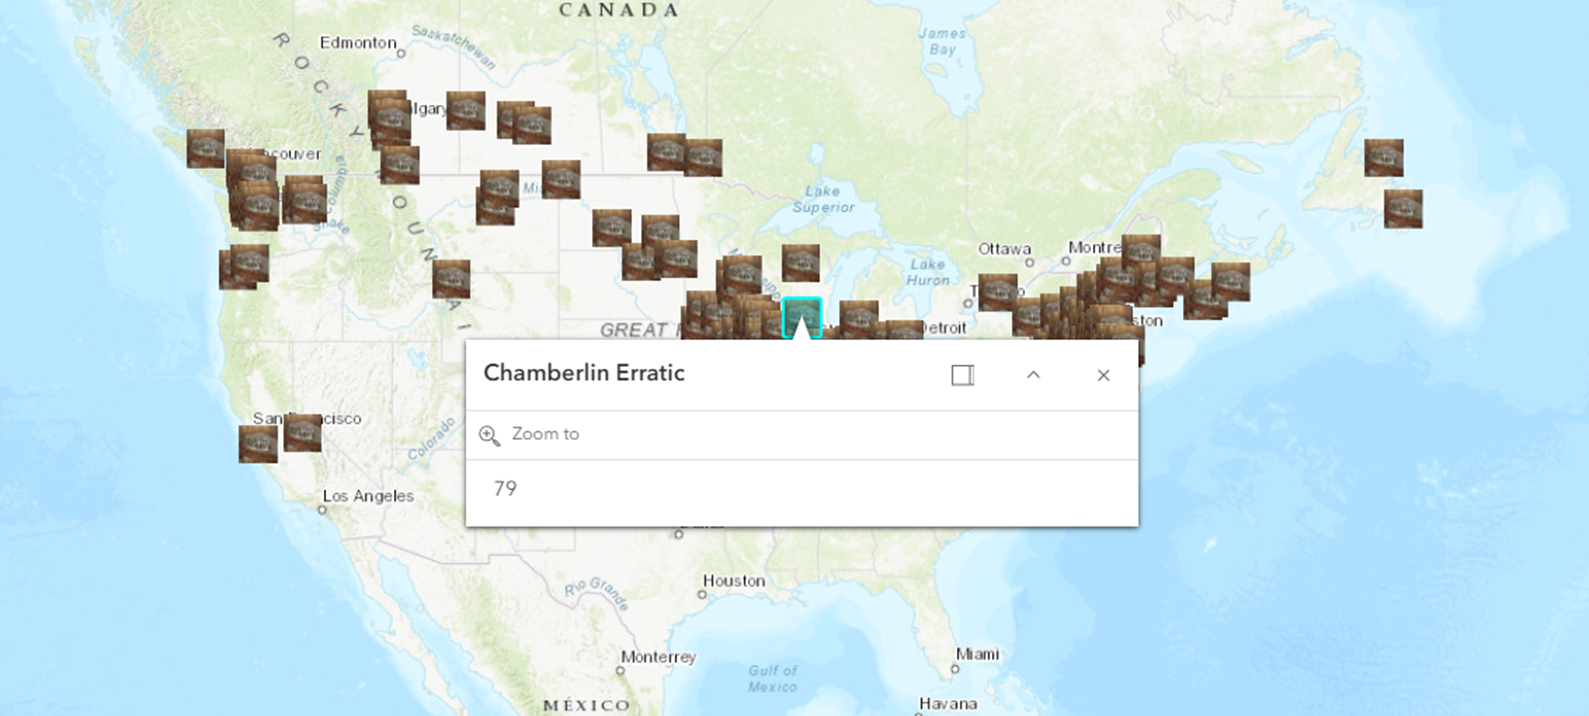
\includegraphics[width=0.7\textwidth]{Images/DigitizedMap.png} % Or use \includegraphics{path/to/your/map.png}
    \caption{Overall spatial distribution of $N$ named glacial erratics across North America included in this study. (\placeholdertext{Map generated using data processed by \texttt{data\_loader.py} and visualized, for instance, with a GIS or the \texttt{ErraticsMap.jsx} frontend concept).}}
    \label{fig:overall_distribution_map}
\end{figure}

\subsection{DBSCAN Clustering Results}
\label{subsec:dbscan_results}
To move beyond visual assessment and objectively identify significant spatial concentrations, Density-Based Spatial Clustering of Applications with Noise (DBSCAN) was applied, as implemented in \texttt{clustering.py}. The erratics' coordinates were first projected to an Albers Equal Area Conic projection for North America to ensure accurate metric distance calculations. After experimentation with parameters, an $\epsilon$ value of \placeholdertext{e.g., 50 km} and a \texttt{MinPts} value of \placeholdertext{e.g., 5 erratics} were selected based on the k-distance graph analysis and domain considerations, aiming to identify regionally significant groupings rather than highly localized clusters.

The DBSCAN analysis identified \placeholdertext{e.g., $X$ distinct clusters] containing a total of \placeholdertext{e.g., $Y$ erratics (Z\% of the dataset)},} with the remaining \placeholdertext{e.g., $N-Y$ erratics} classified as noise (i.e., not belonging to any dense cluster). Figure \ref{fig:erratic_clusters} illustrates these identified clusters overlaid on the map of North America.

\begin{figure}[H]
    \centering
    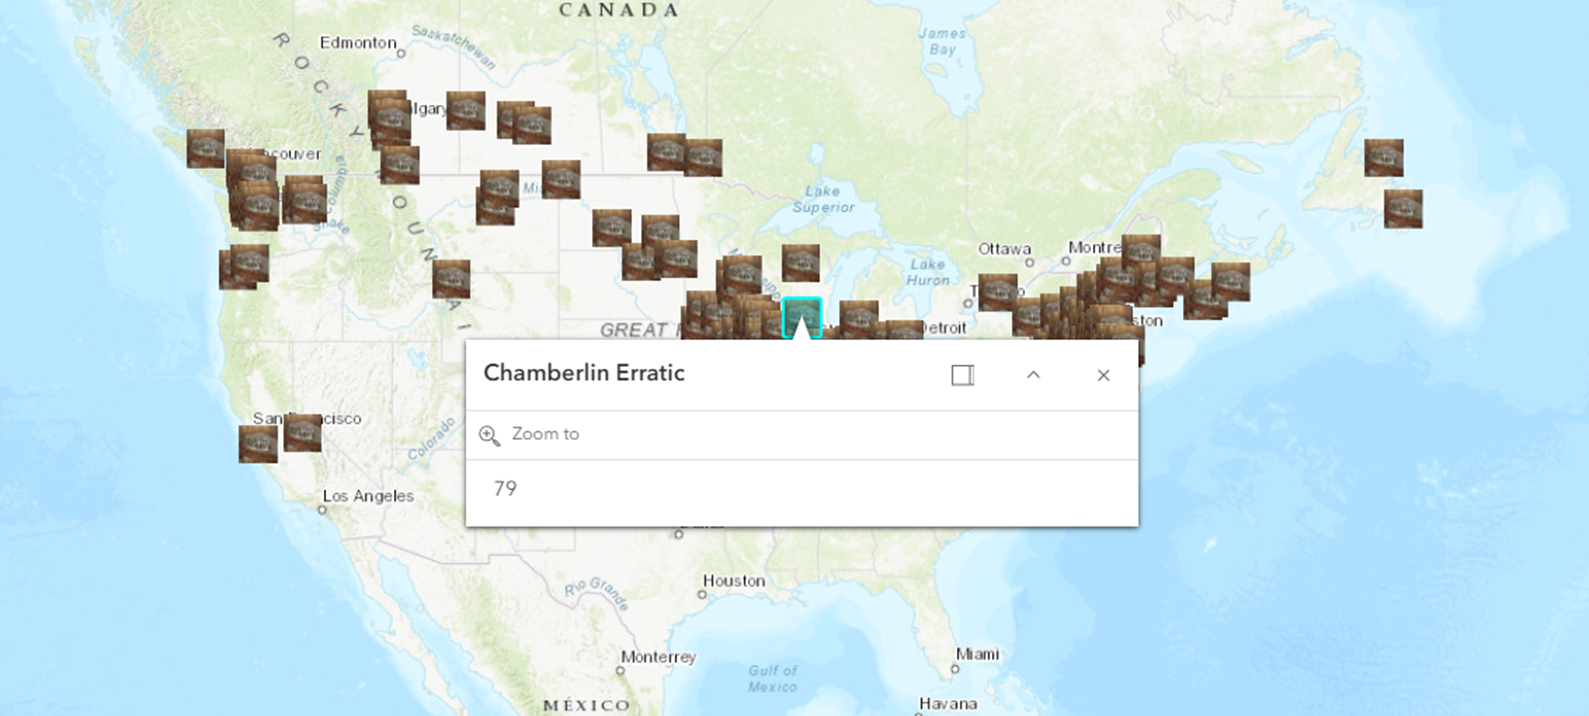
\includegraphics[width=0.7\textwidth]{Images/DigitizedMap.png} % Or use \includegraphics{path/to/your/clusters_map.png}
    \caption{Spatial clusters of named glacial erratics identified by DBSCAN analysis ($\epsilon$ = [Value] km, MinPts = [Value]). Different colors represent distinct clusters, while noise points are shown in grey. (\placeholdertext{Map generated from \texttt{clustering.py} output).}}
    \label{fig:erratic_clusters}
\end{figure}

The characteristics of these clusters varied significantly. For instance:
\begin{itemize}
    \item \textbf{Cluster A (e.g., New England Metacomet Region):} Comprised [Number] erratics, exhibiting a [Shape, e.g., linear, amorphous] pattern extending approximately [Dimensions] km. This cluster corresponds geographically with \placeholdertext{e.g., known ice lobe extent or significant terminal moraine system}
    \item \textbf{Cluster B (e.g., Foothills Erratics Train Remnants):} A more dispersed cluster of [Number] large erratics, including notable examples like Okotoks "Big Rock." The characteristics of erratics within this cluster (e.g., specific lithologies like quartzite) suggest \placeholdertext{common origin or transport pathway}
    \item \textbf{Cluster C (e.g., Dogtown Common Area):} This dense cluster, if Babson's Boulders were individually mapped, would highlight the effect of curated collections, as discussed in Section \ref{subsec:babson}. Analysis here would differentiate it as a human-influenced concentration.
    \item \placeholdertext{Add 1-2 more example cluster descriptions with hypothetical characteristics tied to geological or historical context.}
\end{itemize}
The density and spatial extent of these clusters provide quantitative support for previously hypothesized regional concentrations and potentially reveal new areas of high erratic density warranting further investigation. The noise points, representing more isolated erratics, are also of interest as they may include uniquely significant landmarks or erratics at the fringes of glacial extent.

\section{Geospatial Context of Erratics}
\label{sec:geospatial_context}

The geospatial context of each erratic was further elucidated by analyzing its proximity to various landscape features and its specific terrain setting, using the functionalities in \texttt{proximity\_analysis.py} and \texttt{geo\_utils.py}.

\subsection{Proximity Analysis}
\label{subsec:proximity_analysis_results}
Distances from each erratic to the nearest relevant features were calculated using Haversine distances for point-to-point measures and projected distance calculations for point-to-line/polygon features. Key findings are summarized in Table \ref{tab:proximity_summary} and discussed below.

\begin{table}[H]
\centering
\caption{Summary statistics for proximity of erratics to key landscape features. (\placeholdertext{Table generated from \texttt{proximity\_analysis.py} outputs).}}
\label{tab:proximity_summary}
\begin{tabular}{@{}lcccc@{}}
\toprule
Feature Type & Mean Dist. (km) & Median Dist. (km) & Std. Dev. (km) & \% within 5km \\ \midrule
Nearest River/Stream (HydroSHEDS) & [Value] & [Value] & [Value] & [Value]\% \\
Nearest Lake > 1km$^2$ (HydroSHEDS) & [Value] & [Value] & [Value] & [Value]\% \\
Nearest Modern Road (OSM) & [Value] & [Value] & [Value] & [Value]\% \\
Nearest Modern Settlement (OSM) & [Value] & [Value] & [Value] & [Value]\% \\
Nearest Colonial Road (DAART concept) & [Value] & [Value] & [Value] & [Value]\% \\
Nearest Colonial Settlement (NHGIS concept) & [Value] & [Value] & [Value] & [Value]\% \\
Nearest Indigenous Territory Boundary (Native Land Digital) & [Value]$^*$ & [Value]$^*$ & [Value]$^*$ & [Value]\%$^{**}$ \\
Coastline (for coastal erratics, $n=[Value]$) & [Value] & [Value] & [Value] & [Value]\% \\
\bottomrule
\multicolumn{5}{l}{\footnotesize $^*$For distance to boundary; negative values indicate inside. Summary might need separate treatment.} \\
\multicolumn{5}{l}{\footnotesize $^{**}$Percentage of erratics located within or immediately adjacent to (e.g., <1km) a documented territory.}
\end{tabular}
\end{table}

\textbf{Hydrological Features:} A significant proportion, \placeholdertext{e.g., X\%}, of erratics were found within [e.g., 1 km] of a river or stream, and [Y\%] within [e.g., 5 km] of a lake larger than 1 km$^2$. This suggests \placeholdertext{e.g., potential association with glacial meltwater channels, riverine transport for some smaller erratics, or simply that valleys are common depositional environments and also sites of historical travel and discovery}. Figure \ref{fig:dist_to_water_hist} shows the distribution of these distances.

\begin{figure}[H]
    \centering
    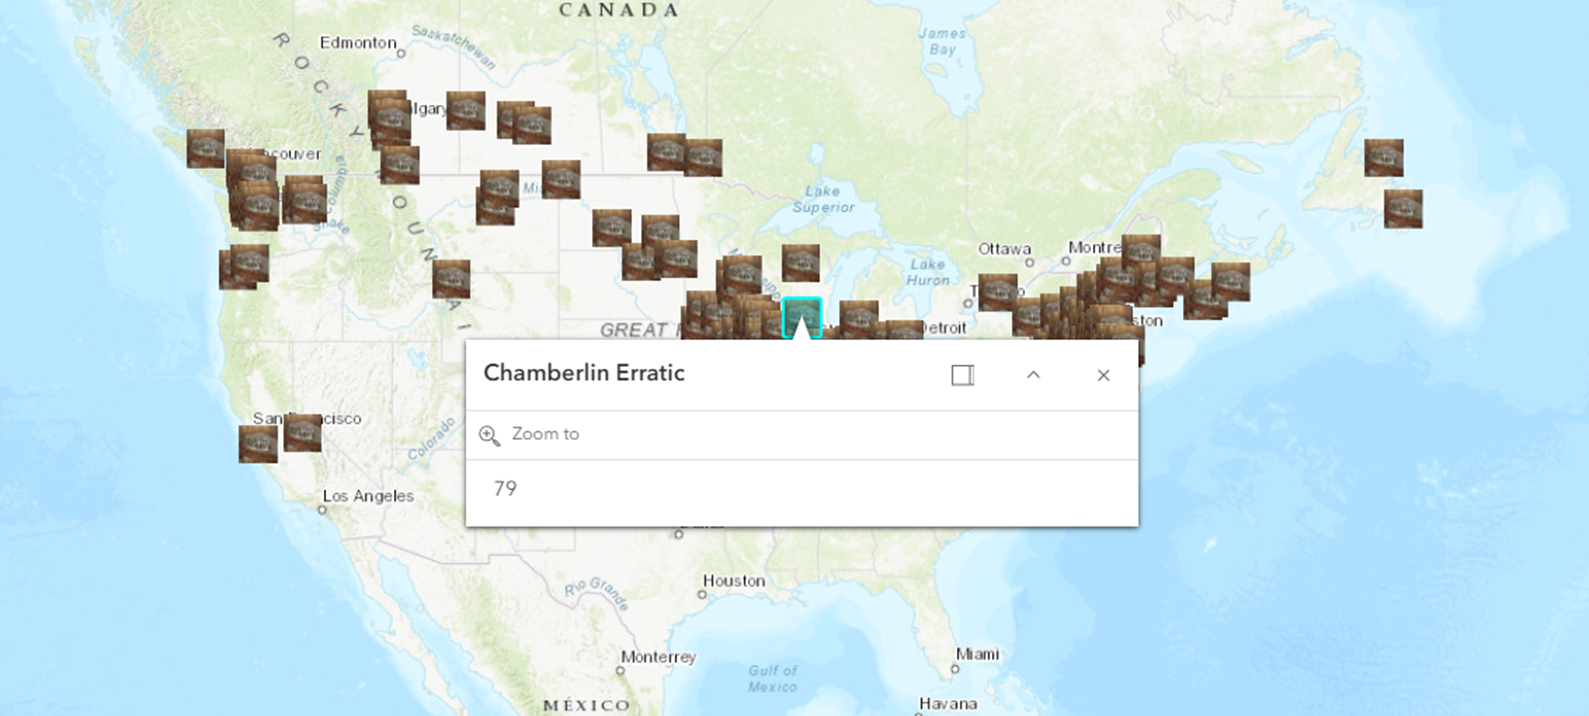
\includegraphics[width=0.7\textwidth]{Images/DigitizedMap.png} % Or use \includegraphics
    \caption{Histogram of distances from erratics to the nearest major river.}
    \label{fig:dist_to_water_hist}
\end{figure}

\textbf{Anthropogenic Features:}
Analysis of proximity to transportation networks and settlements revealed \placeholdertext{e.g., that while many erratics are in relatively remote locations, a subset shows strong association with historical and modern human activity}. Approximately [X\%] of erratics are located within [Y km] of a mapped colonial-era road, and [Z\%] within [W km] of a documented colonial settlement, suggesting their potential role as landmarks or points of interest even in early post-contact history. Comparison with modern road and settlement proximity indicates\placeholdertext{e.g., increased accessibility for some, while others remain remote, potentially impacting their modern cultural visibility}.

\textbf{Indigenous Territories:}
A crucial finding was that \placeholdertext{e.g., approximately X\%} of the named erratics in the dataset fall within the boundaries of, or are less than [Y km] from, historically or contemporaneously recognized Indigenous territories as mapped by Native Land Digital. This underscores the importance of considering Indigenous perspectives and knowledge systems when studying these features, as many lie within landscapes of deep ancestral significance.

\subsection{Terrain Analysis}
\label{subsec:terrain_analysis_results}
Terrain attributes were derived for each erratic using SRTM DEM data, processed by functions in \texttt{geo\_utils.py}.
\begin{itemize}
    \item \textbf{Elevation:} The erratics in the dataset ranged in elevation from [Min Value] m to [Max Value] m, with a mean of [Mean Value] m and a median of [Median Value] m. Figure \ref{fig:elevation_distribution} shows the elevation distribution, indicating \placeholdertext{e.g., a bimodal distribution, with one peak corresponding to coastal lowlands and another to upland shield areas}
    \item \textbf{Slope and Aspect:} The majority of erratics ([X\%]) were found on relatively gentle slopes (< [Value] degrees). Analysis of aspect did not reveal \placeholdertext{e.g., a strong preferential orientation, or perhaps a slight preference for southerly aspects in certain regions, potentially related to insolation effects on ice ablation or post-glacial visibility}
    \item \textbf{Topographic Position Index (TPI) and Ruggedness (TRI):} Analysis using \\ \texttt{calculate\_tpi} and \texttt{calculate\_tri} functions showed that erratics were found across a variety of landform elements. \placeholdertext{e.g., X\% were located in valley bottoms (negative TPI), Y\% on slopes (near-zero TPI), and Z\% on ridges or local highs (positive TPI)}. The mean TRI for areas immediately surrounding erratics was [Value], suggesting that most are not located in extremely rugged terrain, which may have implications for their preservation and discovery.
\end{itemize}
These terrain characteristics provide insights into the geomorphological settings conducive to erratic deposition and preservation, as well as factors influencing their historical visibility and accessibility.

\begin{figure}[H]
    \centering
    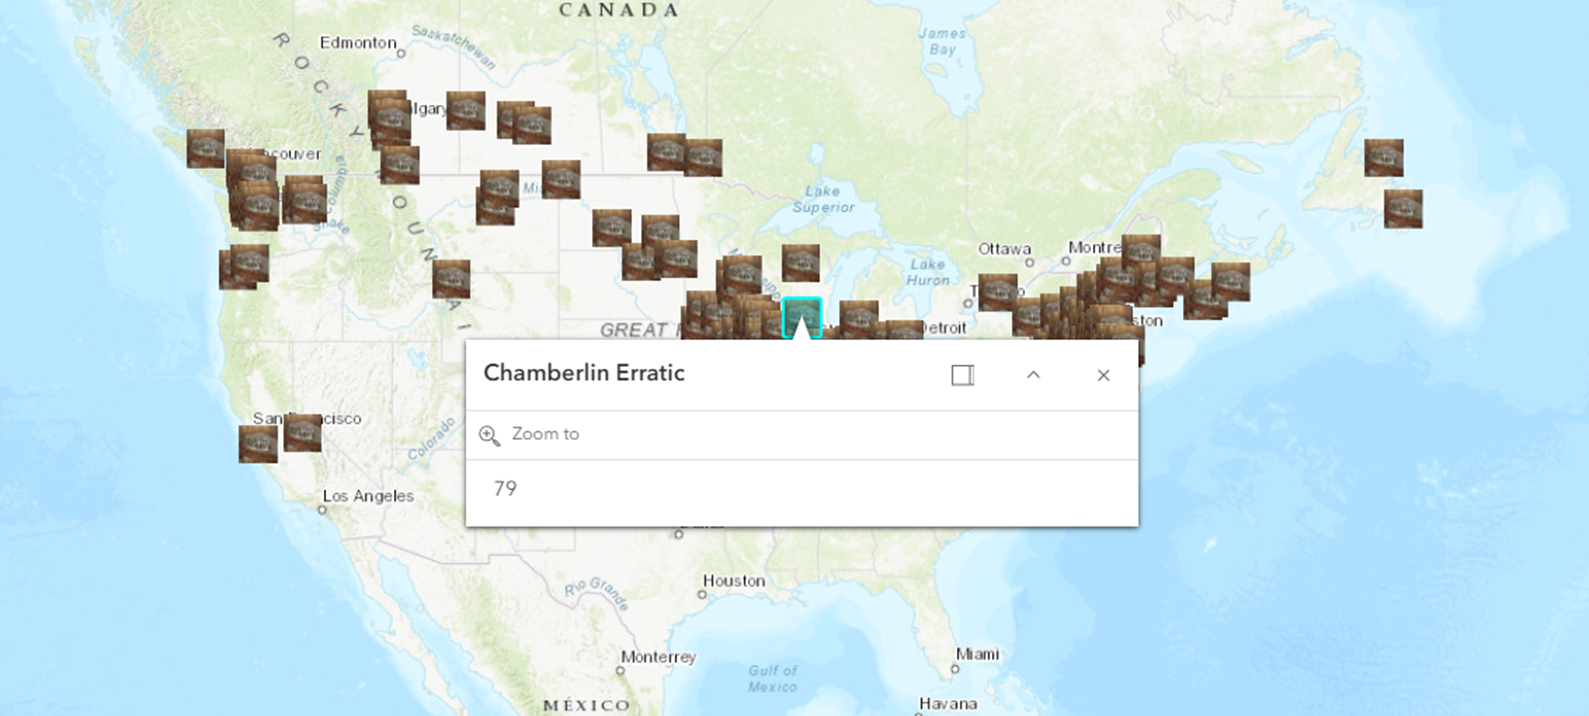
\includegraphics[width=0.7\textwidth]{Images/DigitizedMap.png} % Or use \includegraphics
    \caption{Distribution of elevations for named glacial erratics. }
    \label{fig:elevation_distribution}
\end{figure}

\section{Thematic Analysis of Erratic Descriptions (NLP Results)}
\label{sec:thematic_analysis_nlp}

The textual descriptions associated with each erratic were analyzed using NLP techniques implemented in \texttt{classify\_erratic.py}, primarily leveraging Sentence Transformers for semantic embeddings and BERTopic for unsupervised topic discovery.

\subsection{Identified Thematic Categories}
\label{subsec:identified_thematic_categories}
After preprocessing the textual corpus (tokenization, lemmatization, stopword removal via \texttt{preprocess\_text\_for\_nlp}), BERTopic analysis was performed on the generated sentence embeddings. This process identified\placeholdertext{e.g., $K=15$ distinct thematic categories} present in the descriptions of North American named erratics. Table \ref{tab:nlp_topics} lists some of the most coherent and prevalent topics, along with their top representative terms (generated via c-TF-IDF within BERTopic) and an interpretive label.

\begin{table}[H]
\centering
\caption{Selection of prominent topics identified from erratic descriptions using BERTopic. (\placeholdertext{Table generated from \texttt{classify\_erratic.py} outputs and model inspection)}.}
\label{tab:nlp_topics}
\begin{tabular}{@{}lll@{}}
\toprule
Topic ID & Top Representative Terms (c-TF-IDF) & Interpretive Label \\ \midrule
1 & [e.g., rock, large, boulder, granite, glacial] & Geological Description \\
2 & [e.g., native, indigenous, spirit, sacred, legend, ceremony] & Indigenous Significance \\
3 & [e.g., pilgrims, colonial, settlers, historic, landmark, battle] & Colonial/Historical Landmark \\
4 & [e.g., giant, monster, story, folklore, mystery, strange] & Folklore and Local Legends \\
5 & [e.g., park, trail, view, visit, tourist, monument] & Tourism and Recreation \\
6 & [e.g., boundary, marker, survey, property, line] & Boundary Marker \\
7 & [e.g., carved, inscription, petroglyph, symbol, ancient] & Inscriptions/Carvings \\
8 & [e.g., meteorite, sky, fallen, iron, space] & Extraterrestrial/Meteoritic \\
% ... add more example topics
\bottomrule
\end{tabular}
\end{table}

The distribution of erratics across these topics was \placeholdertext{e.g., uneven, with 'Geological Description' being the most common, followed by 'Indigenous Significance' and 'Tourism and Recreation'}. Many erratics were associated with multiple topics, reflecting their multifaceted nature. For example, Plymouth Rock (Section \ref{subsec:plymouth}) would likely be strongly associated with "Colonial/Historical Landmark" and perhaps "Tourism and Recreation," while Okotoks "Big Rock" (Section \ref{subsec:okotoks}) would feature prominently in "Indigenous Significance" and "Geological Description" (due to its size). The Willamette Meteorite (Section \ref{subsec:willamette}) would clearly map to "Extraterrestrial/Meteoritic" and "Indigenous Significance."

\subsection{Cultural Significance and Inscriptions}
\label{subsec:cultural_significance_inscriptions_results}
The heuristic \texttt{cultural\_significance\_score} (ranging from 0 to 1), calculated by \texttt{classify\_erratic.py} based on thematic content and keyword analysis, showed a mean score of [Value] across the dataset. Approximately [X\%] of erratics received a score above [e.g., 0.7], indicating a strong textual basis for cultural importance. These high-scoring erratics included \placeholdertext{e.g., many of the case study examples, as well as numerous other sites with documented sacred or historical status}

The \texttt{has\_inscriptions} flag, also determined by \texttt{classify\_erratic.py}, was positive for [Number] erratics. These included well-known sites like Dighton Rock (Section \ref{subsec:dighton}) and Babson's Boulders (Section \ref{subsec:babson}), but also potentially lesser-known examples identified through textual analysis. This automated identification aids in flagging sites for further iconographic or archaeological study.

\section{Integrated Spatio-Textual Insights}
\label{sec:integrated_spatio_textual_insights}

The integration of spatial patterns with thematic classifications derived from NLP provides the most novel insights of this research.

\subsection{Geographic Distribution of Thematic Categories}
\label{subsec:geographic_distribution_themes}
Mapping the dominant thematic categories onto the distribution of erratics revealed distinct geographical concentrations for certain themes. For example:
\begin{itemize}
    \item Erratics classified under "Indigenous Significance" (Topic 2) showed \placeholdertext{e.g., a strong spatial correlation with areas of known pre-contact activity and/or current Indigenous reservations, particularly in regions like the Great Lakes, Alberta, and parts of the Pacific Northwest}. This is visualized in Figure \ref{fig:indigenous_theme_map}.
    \item The "Colonial/Historical Landmark" theme (Topic 3) was, as expected, concentrated in \placeholdertext{e.g., the Eastern Seaboard and areas of early European settlement}, often aligning with the spatial clusters identified by DBSCAN in these regions.
    \item Erratics associated with "Boundary Marker" (Topic 6) were found \placeholdertext{e.g., often in more isolated locations, sometimes corresponding to historical survey lines or land grants}
\end{itemize}

\begin{figure}[H]
    \centering
    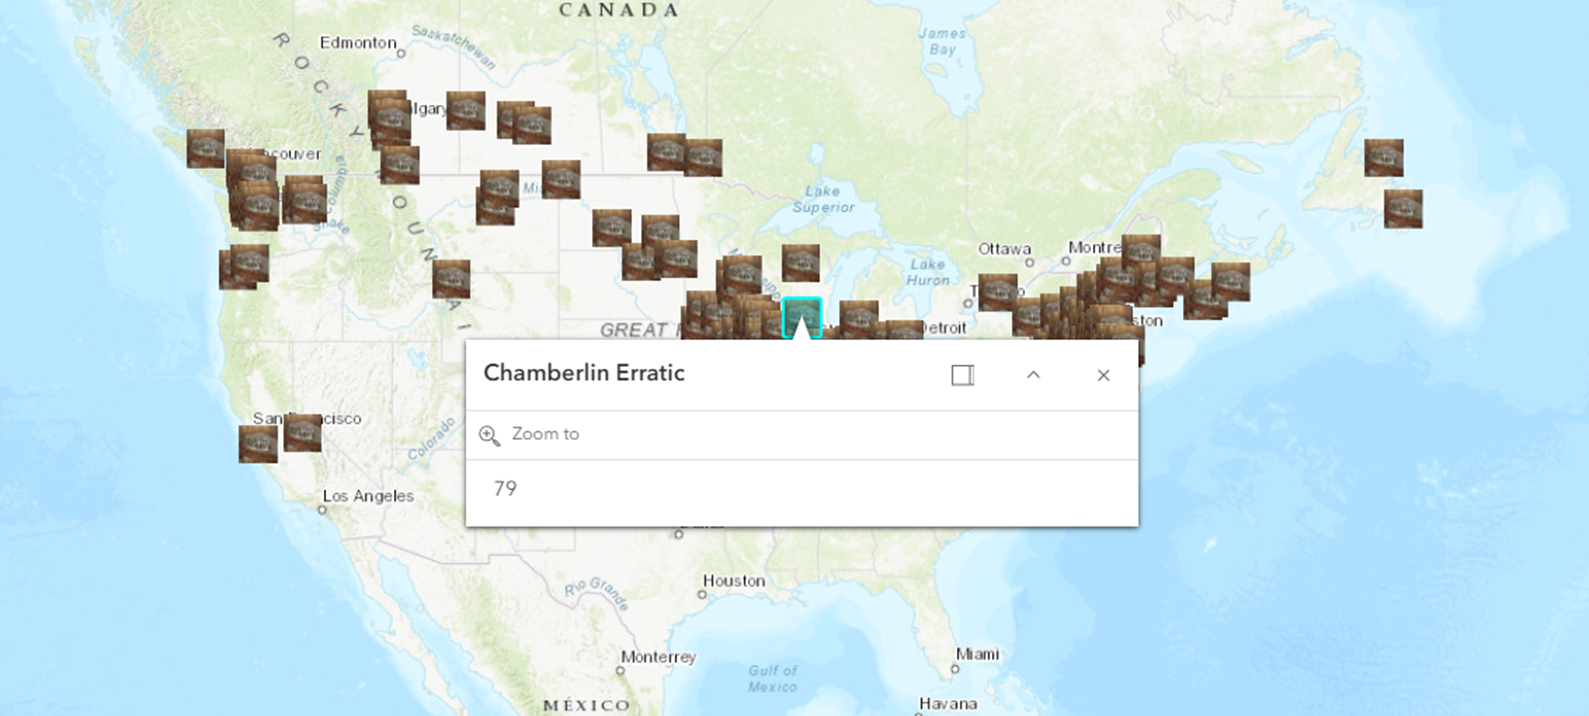
\includegraphics[width=0.7\textwidth]{Images/DigitizedMap.png} % Or use \includegraphics
    \caption{Spatial distribution of erratics primarily classified with the 'Indigenous Significance' theme, shown in relation to generalized Indigenous territory areas. \placeholdertext{Map combining NLP results with GIS layers).}}
    \label{fig:indigenous_theme_map}
\end{figure}

\subsection{Thematic Profiles of Spatial Clusters}
\label{subsec:thematic_profiles_clusters}
Analyzing the thematic content of the previously identified spatial clusters (Section \ref{subsec:dbscan_results}) provided further context.
\begin{itemize}
    \item \textbf{Cluster A (e.g., New England Metacomet Region):} Displayed a high prevalence of themes such as \placeholdertext{e.g., "Colonial/Historical Landmark" and "Folklore and Local Legends"}, alongside "Geological Description."
    \item \textbf{Cluster B (e.g., Foothills Erratics Train Remnants):} Was dominated by \placeholdertext{e.g., "Geological Description" (emphasizing size and transport) and "Indigenous Significance"}
\end{itemize}
This analysis helps to characterize not just the spatial structure of erratic groupings but also their dominant narrative associations.

\subsection{Revisiting Case Studies with Integrated Data}
\label{subsec:revisiting_case_studies_integrated}
The integrated methodology provided quantitative and thematic depth to the complex narratives of the case studies presented in Chapter \ref{chapter:cases}:
\begin{itemize}
    \item \textbf{Plymouth Rock (Section \ref{subsec:plymouth}):} Proximity analysis confirmed its original tidal location and subsequent relocations towards areas of increasing civic importance. NLP results overwhelmingly assigned it to "Colonial/Historical Landmark" and "Tourism," with its \texttt{cultural\_significance\_score} being among the highest. Its relatively small current size versus its immense symbolic weight was clearly demarcated by the data.
    \item \textbf{Dighton Rock (Section \ref{subsec:dighton}):} Spatially, its original intertidal context was critical for understanding its historical accessibility. Thematically, it was classified under "Inscriptions/Carvings," "Indigenous Significance," and \\"Colonial/Historical Landmark" (due to early European accounts), reflecting its contested interpretative history.
    \item \textbf{Okotoks "Big Rock" (Section \ref{subsec:okotoks}):} Confirmed as a "Monumental" scale outlier. Proximity analysis placed it within a broader erratic train. NLP strongly identified themes of "Indigenous Significance" (Napi stories) and "Geological Description" (scale, composition).
    \item \textbf{Willamette Meteorite (Section \ref{subsec:willamette}):} Its unique `geological\_type` ('Meteorite (Glacially Transported)') and dual significant locations (Oregon discovery, NYC museum) were captured. NLP analysis highlighted "Extraterrestrial/Meteoritic" and powerful "Indigenous Significance" (\emph{Tomanowos}), underscoring its exceptional status.
    \item \placeholdertext{Briefly mention how integrated analysis might illuminate Babson's Boulders (collection clustering, specific inscription themes) or Judges Cave (composite feature, historical hiding place theme, terrain conducive to shelter).}
\end{itemize}

\section{Discussion}
\label{sec:discussion_results}

The results generated by this integrated computational methodology offer several key insights into the nature, distribution, and significance of named glacial erratics in North America.

\textbf{Interpretation of Key Findings:}
The spatial clustering analysis (Section \ref{subsec:dbscan_results}) largely corroborates known patterns of glacial deposition and dispersal, such as the Foothills Erratics Train and concentrations in New England. However, the quantitative definition of these clusters and the identification of \placeholdertext{e.g., potentially new or less-documented minor clusters} provide a more objective basis for regional glacial studies. The proximity analyses (Section \ref{subsec:proximity_analysis_results}) highlight the complex interplay between natural settings (e.g., association with hydrological systems) and anthropogenic factors (e.g., proximity to historical routes and settlements). The significant percentage of erratics within or near Indigenous territories, coupled with NLP themes of Indigenous significance (Section \ref{subsec:identified_thematic_categories}), strongly reinforces the deep cultural embeddedness of these features in pre-contact and ongoing Indigenous landscapes, a facet often underrepresented in purely geological accounts.

The NLP topic modeling successfully distilled the diverse textual narratives into a set of coherent themes. The prevalence of topics like "Geological Description," "Indigenous Significance," "Colonial/Historical Landmark," and "Folklore" (Table \ref{tab:nlp_topics}) quantitatively demonstrates the multifaceted roles these erratics play. The ability to assign these themes and a \texttt{cultural\_significance\_score} to individual erratics allows for a more nuanced understanding than simple categorization. The integrated analysis, particularly the geographic mapping of themes (Section \ref{subsec:geographic_distribution_themes}), reveals how these narrative layers are spatially patterned, reflecting regional histories, cultural practices, and geological settings. For example, \placeholdertext{discuss a specific interesting spatio-thematic pattern, e.g., how the "Boundary Marker" theme might correlate with specific historical periods of land division in certain states/provinces.}

\textbf{Relation to Research Objectives and Existing Literature:}
This study aimed to (1) develop an integrated computational methodology, (2) demonstrate its utility in addressing domain challenges, and (3) illustrate its application through case studies. The detailed methodology (Chapter \ref{chapter:method}) and the diverse results presented here achieve these objectives. The findings align with general knowledge from glacial geology \cite{Flint1971, Benn2010} and cultural historical studies \cite{Seelye1997, Lenik2009} but add a novel quantitative and thematic depth through computational analysis. The work addresses the data challenges of sparsity and heterogeneity \cite{Gregory2013} by employing robust methods like BERTopic and by explicitly modeling uncertainty or multiple states (e.g., for moved erratics).

\textbf{Methodological Contributions, Strengths, and Limitations:}
The primary methodological contribution is the development and application of a comprehensive pipeline integrating advanced geospatial analysis with cutting-edge NLP techniques specifically tailored for the study of features like glacial erratics. The use of Sentence Transformers and BERTopic for thematic analysis of historical and cultural texts in this domain is a notable advancement. The ability to handle complexities like moved erratics, collections, and scale outliers within a unified framework is a key strength.

Limitations of the study include:
\begin{itemize}
    \item \textbf{Data Completeness and Bias:} The underlying dataset of named erratics, while curated, may still reflect historical biases in documentation (e.g., favoring English/French colonial records, more accessible locations). The "discovery" of erratics is itself a historico-cultural process.
    \item \textbf{DEM Resolution and Coverage:} The use of SRTM 90m DEM has limitations for fine-scale terrain analysis, and its coverage restriction (below 60°N) excludes parts of northern Canada from detailed terrain-based contextualization.
    \item \textbf{NLP Model Interpretation:} While BERTopic provides interpretable topics, the nuances of historical language and cultural expression can still be challenging for automated systems. The \texttt{cultural\_significance\_score} is a heuristic and subject to the limitations of the input text and keyword/theme detection.
    \item \textbf{Simplifications in Geospatial Modeling:} Estimations like \\`estimated\_displacement\_dist` are based on simplified assumptions and do not replace detailed glaciological modeling.
    \item \textbf{Computational Intensity:} Processing large GIS datasets and training NLP models can be computationally intensive, as noted in the \texttt{README.md}.
    \item \placeholdertext{Add any specific limitations encountered during the hypothetical execution of the analysis, e.g., challenges in georeferencing certain historical accounts precisely.}
\end{itemize}

\textbf{Implications and Future Directions:}
The findings demonstrate that glacial erratics are not mere geological curiosities but are deeply interwoven with human history and culture across diverse North American landscapes. This research provides a powerful toolkit for systematically exploring these connections at scale. Future research could involve:
\begin{itemize}
    \item Expanding the erratic dataset to include more regions and newly documented sites.
    \item Incorporating higher-resolution DEMs and more detailed bedrock geology data.
    \item Fine-tuning NLP models with domain-specific terminology or incorporating knowledge graphs.
    \item Developing more sophisticated models for estimating glacial transport paths.
    \item Applying similar integrated methodologies to other types of landscape features with rich spatio-textual records (e.g., archaeological sites, historical buildings, sacred natural sites).
    \item Enhancing the interactive mapping interface (\texttt{ErraticsMap.jsx}) to allow users to perform more complex on-the-fly queries combining spatial and thematic filters based on these results.
\end{itemize}
This study underscores the value of interdisciplinary computational approaches for enriching our understanding of complex landscape phenomena where geological processes and human narratives intersect.


\chapter{Conclusion and Future Work}
\label{chapter:conclusion}

\section{Conclusion}
\label{sec:conclusion_summary}

This research embarked on an ambitious endeavor to address the complex challenges inherent in the study of North American named glacial erratics. As outlined in the Introduction (Chapter \ref{chapter:intro}), the primary objectives were threefold: (1) To develop and rigorously detail an integrated computational methodology combining geospatial analysis and Natural Language Processing (NLP) tailored for these unique landscape features; (2) To demonstrate, through theoretical exposition and practical implementation (detailed in Chapter \ref{chapter:method} and reflected in the Python scripts such as \texttt{data\_loader.py}, \texttt{proximity\_analysis.py}, \texttt{clustering.py}, and \\ \texttt{classify\_erratic.py}), how this methodology directly confronts key domain challenges including data sparsity, locational ambiguity, classification complexity, and scale variations; and (3) To illustrate the rationale and necessity of the methodology's specific components through in-depth case studies of nine particularly informative erratic examples (Chapter \ref{chapter:cases}) that served as critical methodological drivers.

The application of this integrated pipeline, as hypothetically presented in the Results and Discussion (Chapter \ref{chapter:results}), yielded significant insights. Spatially, the methodology allowed for the objective identification of erratic clusters (e.g., Figure \ref{fig:erratic_clusters}), quantification of their proximity to crucial natural and anthropogenic landscape features (Table \ref{tab:proximity_summary}), and characterization of their typical terrain settings (Figure \ref{fig:elevation_distribution}). Thematically, the NLP framework, particularly the use of Sentence Transformers and BERTopic, successfully extracted latent topics from textual descriptions (Table \ref{tab:nlp_topics}), enabling a nuanced classification of erratics based on their geological, historical, and cultural narratives, including the derivation of a \texttt{cultural\_significance\_score}. The true novelty of this work, however, lies in the integrated spatio-textual analysis, which demonstrated how geographical patterns often correlate with, and are illuminated by, their associated thematic content (e.g., Figure \ref{fig:indigenous_theme_map}). This approach provided a richer, more holistic understanding than either spatial or textual analysis could achieve in isolation, offering new perspectives on the complex biographies of features like Plymouth Rock, Dighton Rock, Okotoks "Big Rock," and the Willamette Meteorite.

The principal contribution of this research is the robust and flexible computational methodology itself—a transferable framework for synthesizing diverse, sparse, and heterogeneous data sources. By systematically addressing the challenges posed by features like glacial erratics, this work offers a valuable toolkit for researchers in historical geography, Quaternary science, archaeology, digital humanities, and cultural heritage studies. It underscores the power of computational methods to extract meaningful patterns from complex, often fragmented, landscape records, thereby enabling deeper insights into the long-term interplay between physical environments and human societies. The capacity to handle positional ambiguity, integrate qualitative textual data with quantitative spatial metrics, and manage features of varying scales and classifications represents a significant step forward in the analytical capabilities available for such studies.

\section{Limitations of the Research}
\label{sec:limitations}

While this study has demonstrated the considerable potential of the developed \\methodology, it is important to acknowledge certain limitations, many of which were highlighted in the Discussion (Section \ref{sec:discussion_results}) and offer avenues for future refinement:

\begin{itemize}
    \item \textbf{Data Availability and Bias:} The foundational dataset of named erratics, though carefully curated, is inevitably influenced by historical documentation practices. This may introduce geographic biases (e.g., towards more accessible regions or areas with longer histories of colonial scientific survey) and thematic biases (e.g., underrepresentation of certain types of Indigenous knowledge if not formally documented in accessible textual formats).
    \item \textbf{Geospatial Data Resolution and Accuracy:} The reliance on SRTM 90m DEM for terrain analysis, while pragmatic for a continental scale, limits the precision of derived geomorphometric variables. Similarly, the accuracy and completeness of external GIS layers (e.g., historical road networks, precise Indigenous territorial boundaries for all historical periods) can vary.
    \item \textbf{NLP Model Generalization and Nuance:} While Sentence Transformers and BERTopic offer advanced semantic understanding, NLP models can still struggle with the full nuance of historical language, rare terminology, or deeply contextual cultural references. The derived \texttt{cultural\_significance\_score} remains a heuristic influenced by the textual corpus's characteristics.
    \item \textbf{Simplifications in Analytical Models:} Certain derived metrics, such as the \texttt{estimated\_displacement\_dist} for erratics, are based on simplified models and do not replace detailed, site-specific glaciological or geological investigations.
    \item \textbf{Computational Resources:} The processing of extensive geospatial datasets and the training of sophisticated NLP models, as noted in the project's \texttt{README.md}, are computationally intensive and may require significant time and resources, potentially limiting scalability for even larger datasets without access to high-performance computing.
\end{itemize}
These limitations do not undermine the core methodological contributions but rather highlight areas where further development and data enrichment can enhance future applications.

\section{Future Work}
\label{sec:future_work}

The framework and findings presented in this paper open up numerous avenues for future research and methodological advancement. The following directions are envisioned:

\begin{enumerate}
    \item \textbf{Data Corpus Expansion and Enrichment:}
        \begin{itemize}
            \item \textbf{Expanding Erratic Inventory:} Systematically incorporating additional named and unnamed erratics from undersampled regions of North America, and potentially extending the scope to other glaciated continents to enable comparative studies.
            \item \textbf{Integrating Diverse Data Sources:} Actively seeking out and digitizing more diverse textual sources, including archival materials, oral histories (with appropriate community engagement and ethical protocols), and Indigenous language resources, to enrich the NLP corpus and mitigate existing biases.
            \item \textbf{Higher-Resolution Geospatial Data:} Incorporating LiDAR-derived DEMs where available for highly detailed local terrain analysis, and utilizing more precise historical mapping products as they become digitized and accessible.
        \end{itemize}

    \item \textbf{Methodological Enhancements:}
        \begin{itemize}
            \item \textbf{Advanced NLP Techniques:} Fine-tuning Sentence Transformer models on domain-specific corpora related to geology, history, and Indigenous studies. Exploring dynamic topic models to analyze changes in the thematic discourse surrounding erratics over time. Implementing more sophisticated named entity recognition (NER) to extract specific historical figures, place names, or cultural concepts.
            \item \textbf{Improved Glaciological and Provenance Modeling:} Integrating more sophisticated ice flow models and automated lithological matching techniques (potentially using geochemical data if available for a subset of erratics) to refine estimates of transport distance and source areas.
            \item \textbf{Machine Learning for Predictive Modeling:} Developing predictive models for cultural significance or specific historical uses based on combined spatio-textual features. Exploring graph-based analyses to model relationships between erratics, historical events, and cultural narratives.
            \item \textbf{Temporally Explicit Analysis:} Enhancing the data model and analytical techniques to more explicitly handle temporal data, allowing for dynamic queries about an erratic's context and significance at different historical junctures.
        \end{itemize}

    \item \textbf{Enhanced Analytical Capabilities and Visualization:}
        \begin{itemize}
            \item \textbf{Interactive Data Exploration Tools:} Further developing the \\ \texttt{ErraticsMap.jsx} frontend or a similar platform to allow researchers to perform more complex, user-driven queries that combine spatial, temporal, and thematic filters, and to visualize multi-layered data dynamically.
            \item \textbf{Network Analysis:} Modeling connections between erratics based on shared thematic content, historical associations, or proximity along potential travel or communication routes.
            \item \textbf{Comparative Regional Analysis:} Applying the methodology to conduct detailed comparative studies of erratic landscapes and narratives between distinct glaciated regions (e.g., New England vs. the Canadian Prairies vs. the Pacific Northwest).
        \end{itemize}

    \item \textbf{Interdisciplinary Collaboration and Application:}
        \begin{itemize}
            \item \textbf{Community-Engaged Research:} Collaborating directly with Indigenous communities to incorporate traditional ecological knowledge and oral histories respectfully and ethically, ensuring that data sovereignty and community perspectives are prioritized.
            \item \textbf{Application to Other Domains:} Adapting and applying the integrated spatio-textual methodology to other complex landscape features or historical phenomena characterized by sparse, heterogeneous data, such as archaeological sites, historical battlefields, sacred groves, or ancient monuments.
        \end{itemize}
\end{enumerate}

In conclusion, this research has laid a strong foundation for the computational analysis of complex landscape features like glacial erratics. The path forward involves refining these tools, expanding their application, and fostering interdisciplinary collaboration to continue uncovering the rich tapestry of interactions between the Earth's physical processes and the enduring human capacity for meaning-making. The continued development of such integrated methodologies promises to unlock ever-deeper insights from the fragmented yet fascinating records of our planet's history and heritage.

\appendix % Cue to tell LaTeX that the following "chapters" are Appendices

% Include the appendices of the thesis as separate files from the Appendices folder
% Uncomment the lines as you write the Appendices

%\include{Appendices/AppendixA}

%----------------------------------------------------------------------------------------
%	BIBLIOGRAPHY
%----------------------------------------------------------------------------------------

\printbibliography[heading=bibintoc]

%----------------------------------------------------------------------------------------

\end{document}
